%% ============================================================
%% Vorlage für ILS Abschlussarbeit
%% ============================================================
%% Datum: 03.07.2019
%% Autor: Johannes Kuhnert Roca
%% Email: johannes.kuhnert-roca@ils.uni-stuttgart.de
%% ============================================================
%%  ***  HINWEIS
%% ============================================================
%% Voraussetzung:
%% MiKTeX, ActivePerl und ein Latex-Editor, wie z.B. TeXStudio, TeXMaker, TexPad, VS Code, etc.
%%
%% Konfiguration des Latex-Editor:
%%		Kompilierungsschritte bei Erzeugung des PDFs: 1. pdflatex 2. makeglossaries 4. pdflatex
%%		Standard-Bibliographie: Bibtex
%%
%% Getestet auf TeXstudio und TexPad 
%% ============================================================

% Koma - Script Version 3.21
\documentclass[english, a4paper, 11pt, twoside, numbers=noenddot, openright,version=3.21]{scrbook}


%Input Daten
%% ============================================================
%%  ***  LaTeX packages
%% ============================================================

% Page layout
\usepackage{geometry}					% set page layout
\usepackage{setspace}					% set line spacing
\usepackage[automark]{scrlayer-scrpage}	% Koma header and footer package

% Language, coding and font
\usepackage{lmodern}					% Font - as requested by ILS
\usepackage[english]{babel} 			% Language setting (last defined is standard)
\usepackage[T1]{fontenc}				% Hyphenation for words with Umlaute
\usepackage[utf8]{inputenc} 			% Coding for correct display of Umlaute
\usepackage[english]{translator}		% Übersetzer
\usepackage{longtable}					% Tables with page break
\usepackage{tabu}
\usepackage{datetime}

% \usepackage{tcolorbox}                  % Code
% \tcbuselibrary{minted,breakable,xparse,skins}

% Graphics and colors
\usepackage[pdftex]{graphicx}					% Include graphics
\usepackage{epstopdf}							% Include eps graphics
\usepackage{color}								% Colors
\usepackage[svgnames,table,hyperref]{xcolor}	% Advanced colors
\usepackage{pythonhighlight}
\usepackage{wrapfig}                            % Wrap images in text
\usepackage{framed}                             % Gray background for quotes

% Math
\usepackage{amsmath,amsthm}				% Math environment
\usepackage{gensymb}					% Degree symbol

% Floats
\usepackage[section]{placeins}			% Control float placement, \FloatBarrier command
% Other
\usepackage[hyphens]{url}				% URL
\usepackage{hyperref}					% Settings for PDF document
\usepackage{caption}					% for modification caption format
\usepackage{subcaption}                 % For subfigures
\usepackage{csquotes}					% Recommended
\usepackage{pdfpages}					% include PDF pages
\usepackage{lipsum}						% lorem ipsum blindtext
\usepackage{siunitx}					% si einheiten
\usepackage{microtype}					% underfull und overfull box problem minimierung
\usepackage{etoolbox}					% Appendix Buchstabenseitenzahl
\usepackage{caption}					% Bildunterschriften
\usepackage{float}						% In der Lage figures explixit an einer Stelle im Text zu fixieren
\setuptoc{toc}{totoc}                   % Add table of contents to the table of contents
\setuptoc{lof}{totoc}                   % Add list of figures to the table of contents
\setuptoc{lot}{totoc}                   % Add list of tables to the table of contents
\setuptoc{bib}{totoc}                   % Add bibliography to the table of contents
\usepackage{ulem}						% Underline text
\usepackage{paralist}					% Modifikation von Listen
\usepackage{titling}					% \theauthor macro

% Anpassbare Enumerates/Itemizes
\usepackage{enumitem}					% Bsp.: Option "style=nextline" für eine gleichmäßige Einrückung aller Zeilen


% Tabellen
\usepackage{lscape}				% mehrseitige Tabellen
\usepackage{booktabs}			% \toprule \midrule \bottomrule
\usepackage{colortbl}			% farbige Tabellen / Tabellen einfärben
\usepackage{multirow}			% mehrere Zeilen verbinden
\usepackage{array}				% Hilfsmittel zum Setzen von Tabellen und geordneten Texten im Mathematischem Modus

% Literatur
\usepackage
[backend=bibtex,						% Backends Bibtex
style=ieee,								% Bibliogragrafiestil IEEE
natbib=true]							% Kompatibilitätsmodul natbib
{biblatex} 								%
\addbibresource{Bibliography/BiB.bib}	% Dateipfad zur Bib Datei

% Glossaries
\usepackage[
xindy,
nonumberlist, 						%keine Seitenzahlen anzeigen
nopostdot,							%keine Punkte
style=super,						% Style
acronym,     						%ein Abkkürzungsverzeichnis erstellen
toc,          						%Einträge im Inhaltsverzeichnis
section=chapter]      				%im Inhaltsverzeichnis auf section-Ebene erscheinen
{glossaries}

%% ============================================================
%%  ***  Page layout
%% ============================================================
\geometry{% 									
left = 2.5cm, 
right=2.5cm, 
top=1.4cm, 
bottom=1.1cm,
includeheadfoot,								
headsep = \dimexpr2\baselineskip-3mm\relax,		% Abstand der Kopfzeile zum Kontext
footskip = \dimexpr2\baselineskip+4mm\relax,	% Abstand der Fußzeile zum Kontext
bindingoffset=1.5mm, 							% max. halb so groß wie der Buchrücken
%showframe										% Rahmen einblenden
}
\KOMAoptions{parskip=yes}						% keine Einrückungen

%% ============================================================

% korrekter Zeilenabstand - \MSonehalfspacing oder \MSdoublespacing wählbar
% anstatt \singlespacing oder \doublespacing
\makeatletter
\newcommand{\MSonehalfspacing}{%
	\setstretch{1.44}%  default
	\ifcase \@ptsize \relax % 10pt
	\setstretch {1.448}%
	\or % 11pt
	\setstretch {1.399}%
	\or % 12pt
	\setstretch {1.433}%
	\fi
}
\newcommand{\MSdoublespacing}{%
	\setstretch {1.92}%  default
	\ifcase \@ptsize \relax % 10pt
	\setstretch {1.936}%
	\or % 11pt
	\setstretch {1.866}%
	\or % 12pt
	\setstretch {1.902}%
	\fi
}
\makeatother
%\MSonehalfspacing	%Gewählte Option

%% ============================================================

% Workaround für römische Zahlen im Inhaltsverzeichen
% Besonder für große Zahlen die viel Platz einnehmen
\makeatletter% --> De-TeX-FAQ
\renewcommand*{\@pnumwidth}{3em}
\makeatother% --> \makeatletter


%% ============================================================
%%  ***  Header & Footer Layout
%% ============================================================

\KOMAoptions{headsepline=true,	% header line
	footsepline=false,			% footer line
	cleardoublepage=plain,	% set empty pages to style 'plain'
	plainheadsepline=false,	% activate header line for plain pages
	plainfootsepline=false}	% activate footer line for plain pages


\pagestyle{scrheadings}
\clearpairofpagestyles

% The following checks whether \headmark has the width of 0pt, and if so, changes the color of the headsepline to white:
\newcommand*{\specialheadmark}{%
	\setbox0\hbox{\headmark}%
	\ifdim\wd0=0pt\relax%
	\global\setkomafont{headsepline}{\color{white}}%
	\else%
	\global\setkomafont{headsepline}{\color{black}}%
	\fi%
	\unhbox0%
}

% Setzt Textstill im Footer auf normal - kein Kursiv mehr!
\renewcommand*{\footfont}{\normalfont}

\lehead{\specialheadmark}
\rohead{\specialheadmark}
\ofoot*{\pagemark}


% Redeclare Chapter/Sections/... spacing
\RedeclareSectionCommand[beforeskip=1sp, afterskip=10pt]{chapter}
\RedeclareSectionCommands[beforeskip=1sp, afterskip=1sp]{section,subsection,subsubsection}

\renewcommand{\dateseparator}{.}	% Replace Seperator / by .

%% ============================================================
%%  ***  Reference style
%% ============================================================
\captionsetup{tablewithin=chapter}	% Change 'Table 12' to 'Table 2.3' format - as requested by ILS
\captionsetup{figurewithin=chapter}	% Change 'Figure 12' to 'Figure 2.3' format - as requested by ILS

\setcounter{secnumdepth}{3} % Adjust section numbering here
\setcounter{tocdepth}{4}	% Adjust table of contents depth here



%% ============================================================
%%  ***  Glossary Erstellung
%% ============================================================
%Ein eigenes Symbolverzeichnis erstellen
\newglossary[slg]{symbolslist}{syi}{syg}{Symbolverzeichnis}
% Zusätzliches Feld - Einheit - für das Symbolverzeichnis 
\glsaddkey{unit}{\glsentrytext{\glslabel}}{\glsentryunit}{\GLsentryunit}{\glsunit}{\Glsunit}{\GLSunit}
% Option um SI befehle zu nutzen
\glssetnoexpandfield{unit}
%Den Punkt am Ende jeder Beschreibung deaktivieren
\renewcommand*{\glspostdescription}{}
%Glossar-Befehle anschalten
\makeglossaries

% Neuer Style für das Symbolverzeichnis auf Basis des "long3col" Style
%% ============================================================
\newglossarystyle{symbunitlong}{%
	\setglossarystyle{long3col}% base this style on the list style
	\renewenvironment{theglossary}{% Change the table type --> 3 columns
		\begin{longtable}{@{}l l p{0.8\glsdescwidth} @{}c}}%
		{\end{longtable}}%
	%
	\renewcommand*{\glossaryheader}{%  Change the table header
		\bfseries Symbol & \bfseries Beschreibung & & \bfseries Einheit \\
		\hline
		\endhead}
	\renewcommand*{\glossentry}[2]{%  Change the displayed items
		\glstarget{##1}{\glossentryname{##1}} %
		& \glossentrydesc{##1}% Description
		&
		& \glsunit{##1}  \tabularnewline
	}
}
%% ============================================================
%Ende des neuen Styles


%% ============================================================
%%  ***  Custom Item Erstellung für Requirements and Deliverables
%% ===========================================================
% eigener Zähler für Requirements
% Ausgabe mit \requirement und \subrequirement
\newcounter{req}
\newcounter{subreq}[req]

\renewcommand\thesubreq{\thereq.\arabic{subreq}}

\newcommand{\requirement}[1]{%
	REQ~\refstepcounter{req}\thereq~#1}

\newcommand{\subrequirement}[1]{%
	REQ~\refstepcounter{subreq}\thesubreq~#1}


% eigener Zähler für Deliverables
% Ausgabe mit \deliverable und \subdeliverable
\newcounter{del}
\newcounter{subdel}[del]

\renewcommand\thesubdel{\thedel.\arabic{subdel}}

\newcommand{\deliverable}[1]{%
	DEL~\refstepcounter{del}\thedel~#1}

\newcommand{\subdeliverable}[1]{%
	DEL~\refstepcounter{subdel}\thesubdel~#1}

%% ============================================================
%%  ***  User commands
%% ============================================================

\renewcommand{\*}{\cdot}
\newcommand{\tabitem}{~~\llap{\textbullet}~~}


%% ============================================================
%%  ***  User formats
%% ============================================================
% \newcommand{\bold}[1]{\textbf{#1}}


%% ============================================================
%%  ***  Color definitions
%% ============================================================
% \definecolor{yellow}{rgb}{230,248,54}

% Input für Glossar, Abkürzungsverzeichnis und Symbolverzeichnis

%% ============================================================
% Symbolverzeichnis und Einheit
%% ============================================================
\newglossaryentry{symb:Pi}{
name=$\pi$,
description={Die Kreiszahl.},
unit = {-},
sort=symbolpi, type=symbolslist
}
\newglossaryentry{symb:Phi}{
name=$\varphi$,
description={Ein beliebiger Winkel.},
unit = {-},
sort=symbolphi, type=symbolslist
}
\newglossaryentry{symb:Lambda}{
name=$\lambda$,
description={Wellenlänge},
unit = {-},
sort=symbollambda, type=symbolslist
}
\newglossaryentry{symb:alpha}{
name=$\alpha$,
description={Winkel},
unit = {\si{\degree}},
sort=symbolalpha, type=symbolslist
}
\newglossaryentry{symb:beta}{
name=$\beta$,
description={Winkel},
unit = {\si{\degree}},
sort=symbolbeta, type=symbolslist
}
%% ============================================================
%Abkürzungsverzeichnis
%% ============================================================
\newacronym{MS}{MS}{\textbf{M}icro\textbf{s}oft}
\newacronym{CD}{CD}{\textbf{C}ompact \textbf{D}isc}
\newacronym{VW}{VW}{\textbf{V}olks\textbf{w}agen}
\newacronym{VWW}{VWW}{\textbf{V}olks\textbf{w}agen\textbf{w}are}
\newacronym{DVD}{DVD}{DVD}
%Eine Abkürzung mit Glossareintrag
\newacronym{AD}{AD}{\textbf{A}ctive \textbf{D}irectory\protect\glsadd{glos:AD}}

%% ============================================================
%Glossareintrag
%% ============================================================%
\newglossaryentry{glos:AD}{
	name=Active Directory,
	description={Active Directory ist in einem Windows 2000 Windows
		Server 2003-Netzwerk}
}
\newglossaryentry{glos:AntwD}{name=Antwortdatei, description={Informationen zum
		Installieren einer Anwendung oder des Betriebssystems.}}
%Ausgabe aller Symbole	
\glsaddall[types=symbolslist]


\title{Visualization Verification of Complex Avionic Models Using Computer Vision}
\author{Franz Köhler}
\date{07.10.2024}

%% ============================================================
%%  ***  HYPERLINKS for pdfTeX /
%% ============================================================
\hypersetup{
	pdftitle    = {\thetitle},
	pdfsubject  = {Visualization Verification of Complex Avionic Models Using Computer Vision},
	pdfauthor   = {\theauthor},
	pdfkeywords = {bachelorthesis, computervision, python, opencv, uml, verification},
	pdfborder   = 0 0 0,
	plainpages  = false,
	bookmarksnumbered = true,
}

\begin{document}


%% ============================================================
%%  ***  Cover
%% ============================================================
\hypersetup{pageanchor=false}
\pagenumbering{gobble}

\includepdf[pages={1}]{./Cover/cover.pdf}
\cleardoublepage
\hypersetup{pageanchor=true}

%% ============================================================
%%  ***  Preamble
%% ============================================================

\pagenumbering{Roman}

% Sperrvermerk
\addchap*{Sperrvermerk}


Diese vorliegende Abschlussarbeit ist eine nicht öffentliche Version und beinhaltet vertrauliche und interne Daten der MUSTERFIRMA. Sie darf nur der Prüfungskommission der Universität Stuttgart und für das Prüfungsverfahren notwendigen Personen zugänglich gemacht werden. Die Abschrift bzw. Vervielfältigung von Datenmaterial - auch in Auszügen - ob in digitaler oder analoger Form ist nicht gestattet. Eine Ausnahme von dieser Regelung bedarf der schriftlichen Genehmigung des Autors und der MUSTERFIRMA.

% Aufgabenstellung
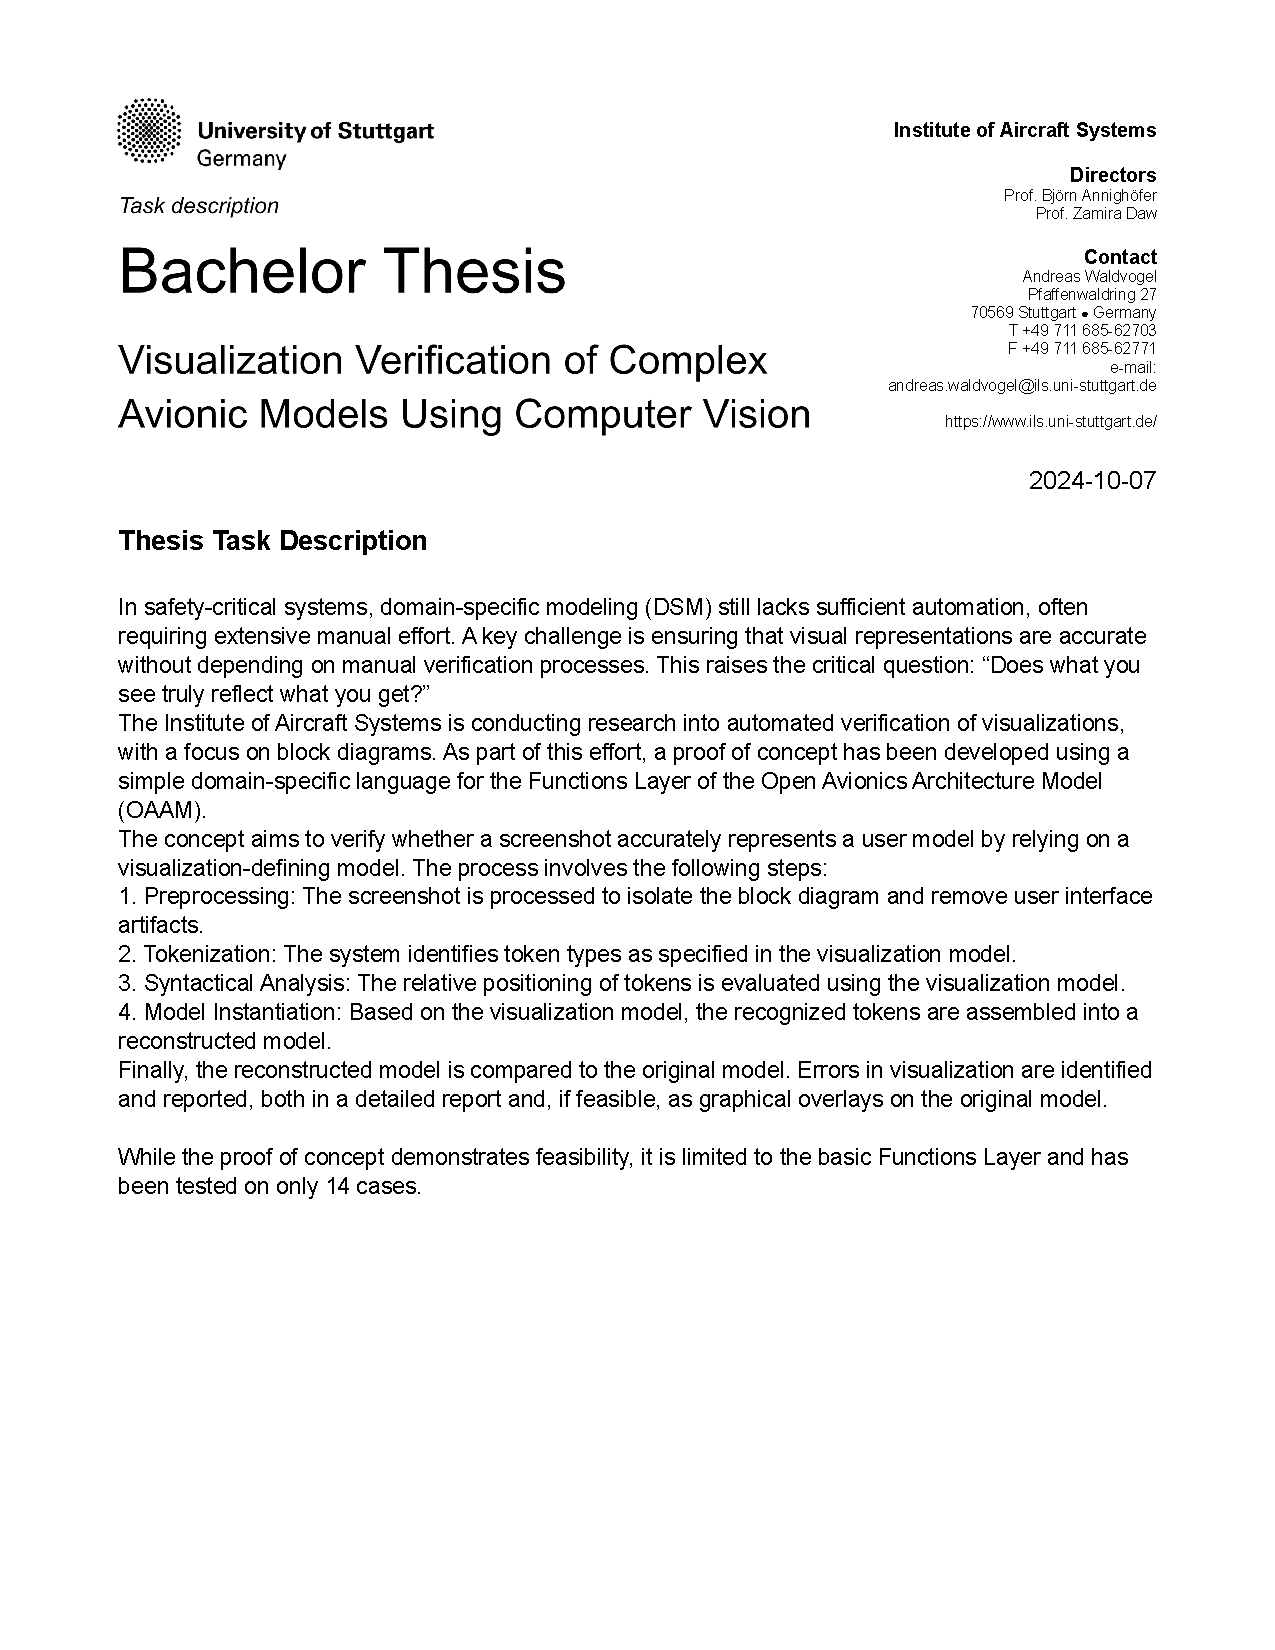
\includepdf[pages={1-3}]{Preamble/task.pdf}

% Erklärung zur selbständigen Arbeit
\addchap*{Selbst{\"a}ndigkeitserkl{\"a}rung}

Hiermit versichere ich, dass ich diese Bachelorarbeit / Masterarbeit selbst{\"a}ndig mit Unterst{\"u}tzung des Betreuers/ der Betreuer angefertigt und keine anderen als die angegebenen Quellen und Hilfsmittel verwendet habe. Die Arbeit oder wesentliche Bestandteile davon sind weder an dieser noch an einer anderen Bildungseinrichtung bereits zur Erlangung eines Abschlusses eingereicht worden.

Ich erkl{\"a}re weiterhin, bei der Erstellung der Arbeit die einschl{\"a}gigen Bestimmungen zum Urheberschutz fremder Beitr{\"a}ge entsprechend den Regeln guter wissenschaftlicher Praxis\footnote{Nachzulesen in den DFG-Empfehlungen zur "`Sicherung guter wissenschaftlicher Praxis"' bzw. in der Satzung der Universit{\"a}t Stuttgart zur "`Sicherung der Integrit{\"a}t wissenschaftlicher Praxis und zum Umgang mit Fehlerverhalten in der Wissenschaft"'} eingehalten zu haben. Soweit meine Arbeit fremde Beitr{\"a}ge (z.B. Bilder, Zeichnungen , Testpassagen etc.) enth{\"a}lt, habe ich diese Beitr{\"a}ge als solche gekennzeichnet (Zitat, Quellenangaben) und eventuell erforderlich gewordenen Zustimmungen der Urheber zu Nutzung dieser Beitr{\"a}ge in meiner Arbeit eingeholt. Mit ist bekannt, dass ich im Falle einer schuldhaften Verletzung dieser Pflichten die daraus entstehenden Konsequenzen zu tragen habe.

\vspace{2cm}

Stuttgart, den \thedate \hfill \rule{8cm}{0.4pt} \linebreak
\mbox{~} \hfill	\theauthor

\addchap*{Nutzungsrechterkl{\"a}rung}

Hiermit erkl{\"a}re ich mich damit einverstanden, dass meine Bachelorarbeit / Masterarbeit zum Thema:
\begin{center}
	\textit{\thetitle}
\end{center}
in der Institutsbibliothek des Institutes f{\"u}r Luftfahrtsysteme mit sofortiger Wirkung {\"o}ffentlich zug{\"a}nglich aufbewahrt und die Arbeit auf der Institutswebseite sowie im Online-Katalog der Universit{\"a}tsbibliothek erfasst wird. Letzteres bedeutet eine dauerhafte, weltweite Sichtbarkeit der bibliographischen Daten der Arbeit (Titel, Autor, Erscheinungsjahr, etc.).

Nach Abschluss der Arbeit werde ich zu diesem Zweck meinem Betreuer neben dem Pr{\"u}fexemplar eine weitere gedruckte sowie eine digitale Fassung {\"u}bergeben.

Der Universit{\"a}t Stuttgart {\"u}bertrage ich das Eigentum an diesen zus{\"a}tzlichen Fassungen und r{\"a}ume dem Institut f{\"u}r Luftfahrtsysteme an dieser Arbeit und an den im Rahmen dieser Arbeit von mir erzeugten Arbeitsergebnissen ein kostenloses, zeitlich und {\"o}rtlich unbeschr{\"a}nktes, einfaches Nutzungsrecht f{\"u}r Zwecke der Forschung und der Lehre ein. Falls in Zusammenhang mit der Arbeit Nutzungsrechtsvereinbarungen des Instituts mit Dritten bestehen, gelten diese Vereinbarungen auch f{\"u}r die im Rahmen dieser Arbeit entstandenen Arbeitsergebnisse.

\vspace{2cm}

Stuttgart, den \thedate \hfill \rule{8cm}{0.4pt} \linebreak
\mbox{~} \hfill	\theauthor





 % 

% Kurzzusammenfassung/Abstract - (1/2 Seite Deutsch, 1/2 Seite Englisch)
\addchap*{Abstract}
\label{abstract}
{\LARGE Visualization Verification of Complex Avionic Models Using Computer Vision}

With the increasing complexity of models and applications in aviation, the use of domain specific modeling (DSM) in the field has become vital. DSM enables engineers to work more efficiently and reduce errors in generated code through automation. However, for use in safety-critical applications, DSM requires significant effort, particularly in ensuring correct model visualizations to reduce the amount of manual verification work.

This thesis aims to build upon the work of \cite{og_paper} to improve the reliability of the automated verification of block-diagram visualizations in DSM. In \cite{og_paper}, the computer vision library \textit{Open Computer Vision} or \textit{OpenCV} was used to recognize and process block diagram models. The results were compared with the original model to find and indicate deviations to the user inside a browser-based graphical model editor called \textit{eXtensible Graphical EMOF Editor} or \textit{XGEE}.
The original implementation of the block diagram recognition algorithm was limited in its ability to process complex and diverse diagrams within XGEE.

This thesis extends the capabilities of the block diagram recognition algorithm to work with complex and diverse diagrams in three seperate graphical domain-specific languages within XGEE. The new implementation is able to correctly identify and process intersecting or partially obscured connecting edges in any orientation, detect a larger variety of overlapping vertices of differing sizes and shapes and process text labels in multiple orientations, showcasing its potential to significantly reduce manual verification effort in DSM applications.
\cleardoublepage
\addchap*{Kurzzusammenfassung}
\label{kurzzusammenfassung}
{\LARGE Verifikation von Visualisierungen von komplexen Avionik Modellen mit Computer Vision}

Mit der steigenden Komplexität von Modellen und Applikationen wird die Nutzung von Domain Specific Modeling (DSM) in der Luftfahrtindustrie immer wichtiger. Es ermöglicht Ingenieuren, effizienter und sicherer zu arbeiten und reduziert duch autmatische Code Generation die Fehleranfälligkeit der fertigen Programme. Bei sicherheitskritischen Anwendungen jedoch ist DSM mit signifikantem Mehraufwand verbunden. Ein wichtiges Problem ist die korrekte visuelle Darstellung des Modells um manuelle verifizierung zu vermeiden.\\
Diese Arbeit baut auf \cite{ar_prof_paper}, um die Sicherheit der automatischen Verifikation von Block-Diagramm-Visualisierungen in DSM zu verbessern. In \cite{ar_prof_paper} werden methoden aus der Computer-Vision genutzt, um Block Diagramme zu erkennen, mit den internen Modellen zu vergleichen und Unterschiede visuell darzustellen. 
\cleardoublepage

% Danksagung
%\include{./Preamble/Danksagung}
%\cleardoublepage


%% ============================================================
%%  ***  Contents and Lists
%% ============================================================
\phantomsection

% Contents
\tableofcontents

% Figures
\listoffigures

% % Tables
% \listoftables
% \cleardoublepage

% %Glossar
% \printglossary[style=super,title=Glossary]
% \cleardoublepage

% % Abbrevations
% \printglossary[type=\acronymtype,title=Index of abbreviations]
% \cleardoublepage

% % Symbols and Units
% \printglossary[type=symbolslist,style=symbunitlong,title={Index of Symbols and Units}]
% \cleardoublepage


%% ============================================================
%%  ***  Chapters
%% ============================================================
\pagenumbering{arabic}
\chapter{Introduction}
\label{chp:introduction}

Development of complex systems requires an efficient way for engineers to ensure the correctness of the developed software. Domain Specific Modeling (DSM) can, through automatic code generation and block-diagram visualizations, significantly reduce the risk of faulty applications, and enable engineers to work more effectively. In safety-critical development processes however, DSM can only be used without subsequent manual verification, if the DSM tools work correctly. This can either be achieved through time intensive qualified software development processes, which ensure accurate and reliable visualization of DSM through the tool itself, or through the use of unverified DSM tools followed by the subsequent use of a small visualization verification tool to ensure the correctness of the application.

In low-cost projects with high safety requirements, a cost-effective qualification method is crucial, highlighting the potential of the latter approach for a qualifiable graphical editing tool for use in DSM.

The Institute for Aircraft Systems is currently developing a way for avionic models to be developed inside a web-based graphical model editor called "eXtensible Graphical EMOF Editor" or "XGEE".\\
XGEE uses three kinds of "tokens" within three distinct editors to visualize avionic models. They are:
\begin{itemize}
    \item signals
    \item vertices
    \item text labels
\end{itemize}
\begin{figure}[h]
    \centering
    % First image
    \begin{subfigure}{0.3\textwidth}
        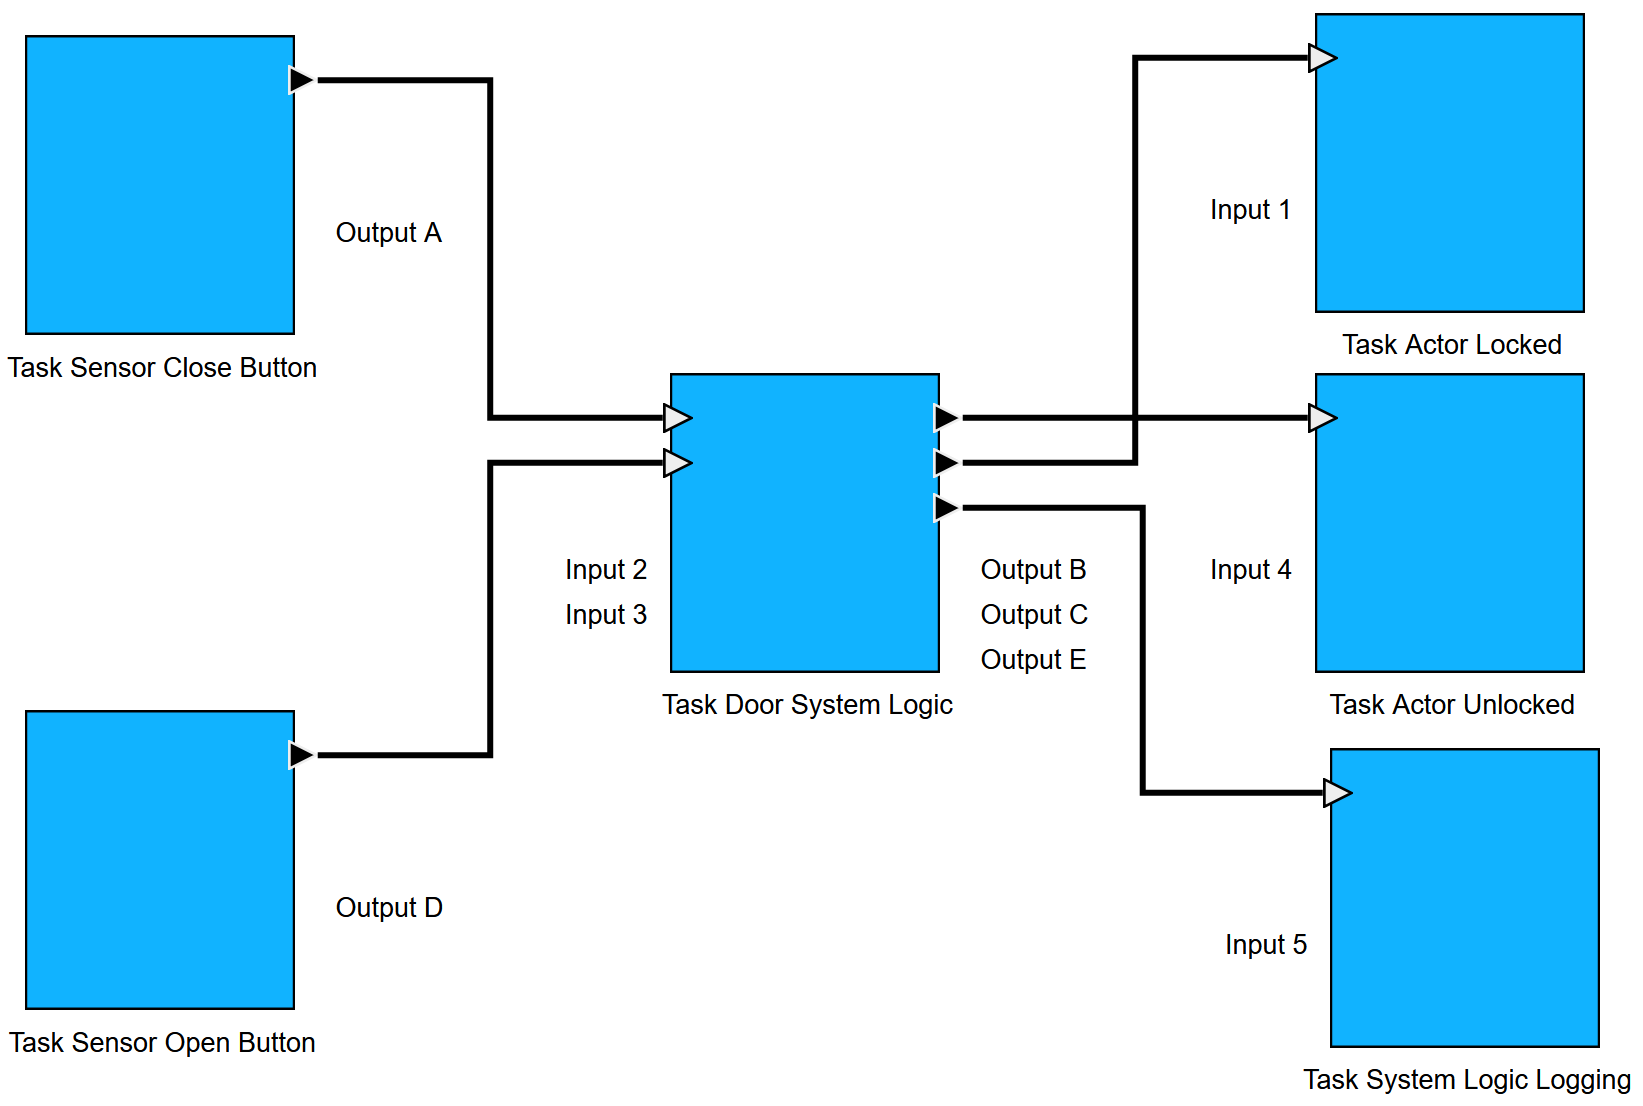
\includegraphics[width=\linewidth]{Pictures/functions_editor.png}
        \caption{Functions editor}
        \label{fig_functions_editor_en}
    \end{subfigure}
    \hfill
    % Second image
    \begin{subfigure}{0.3\textwidth}
        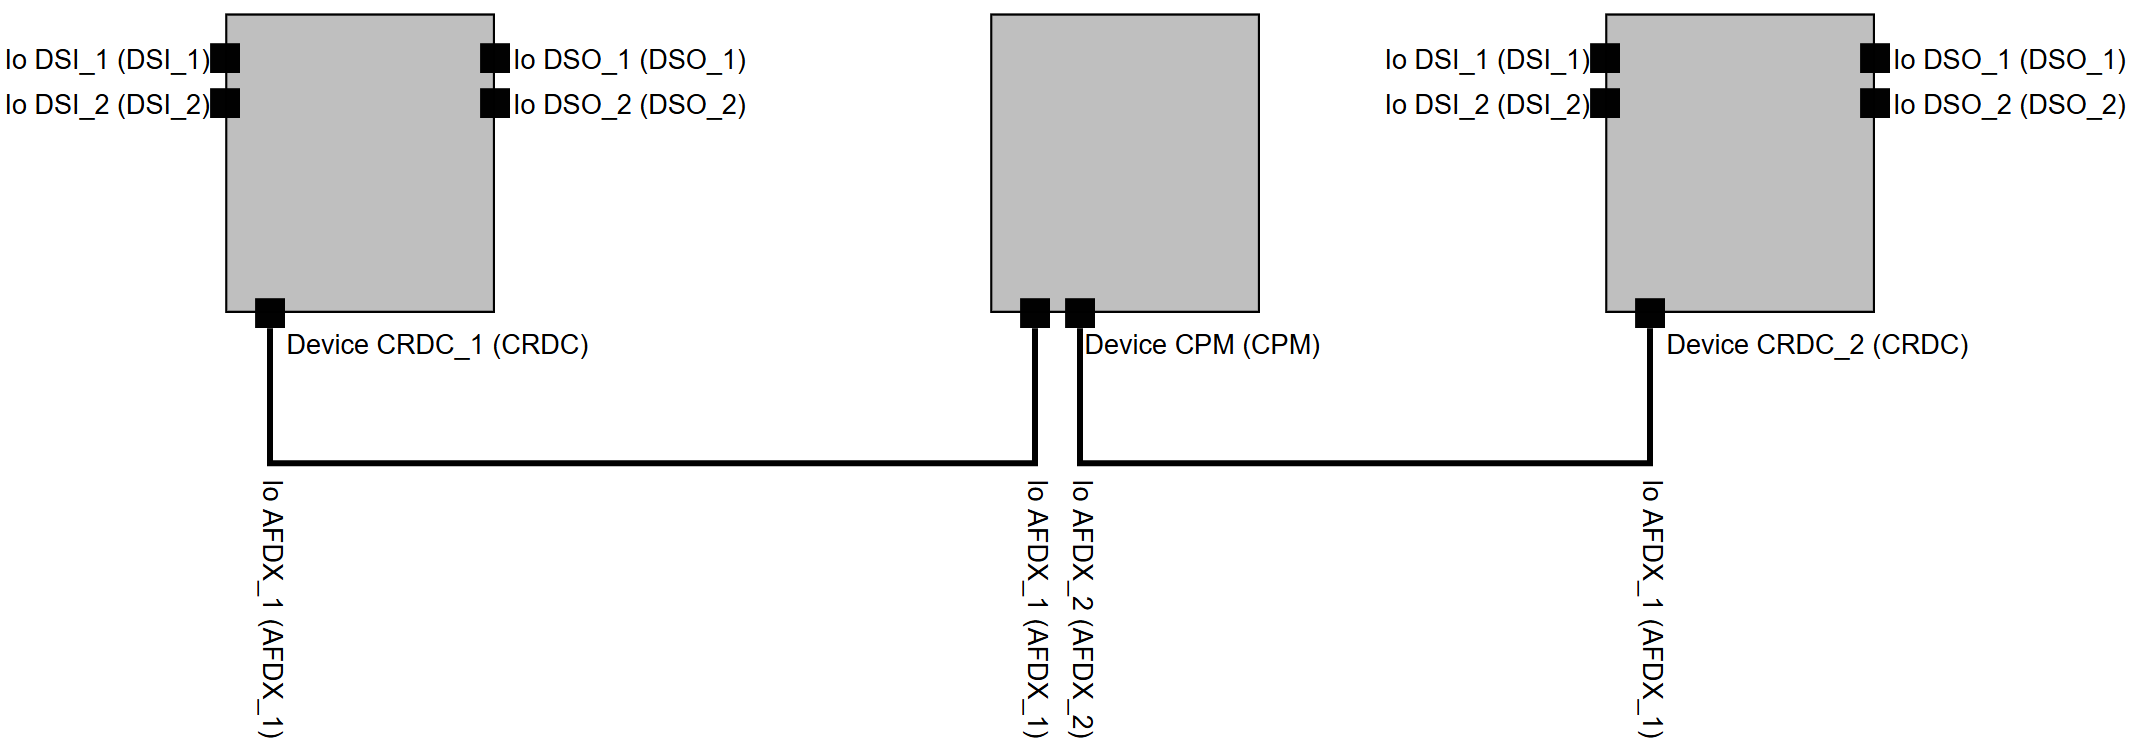
\includegraphics[width=\linewidth]{Pictures/hardware_editor.png}
        \caption{Hardware editor}
        \label{fig_hardware_editor_en}
    \end{subfigure}
    \hfill
    % Third image
    \begin{subfigure}{0.3\textwidth}
        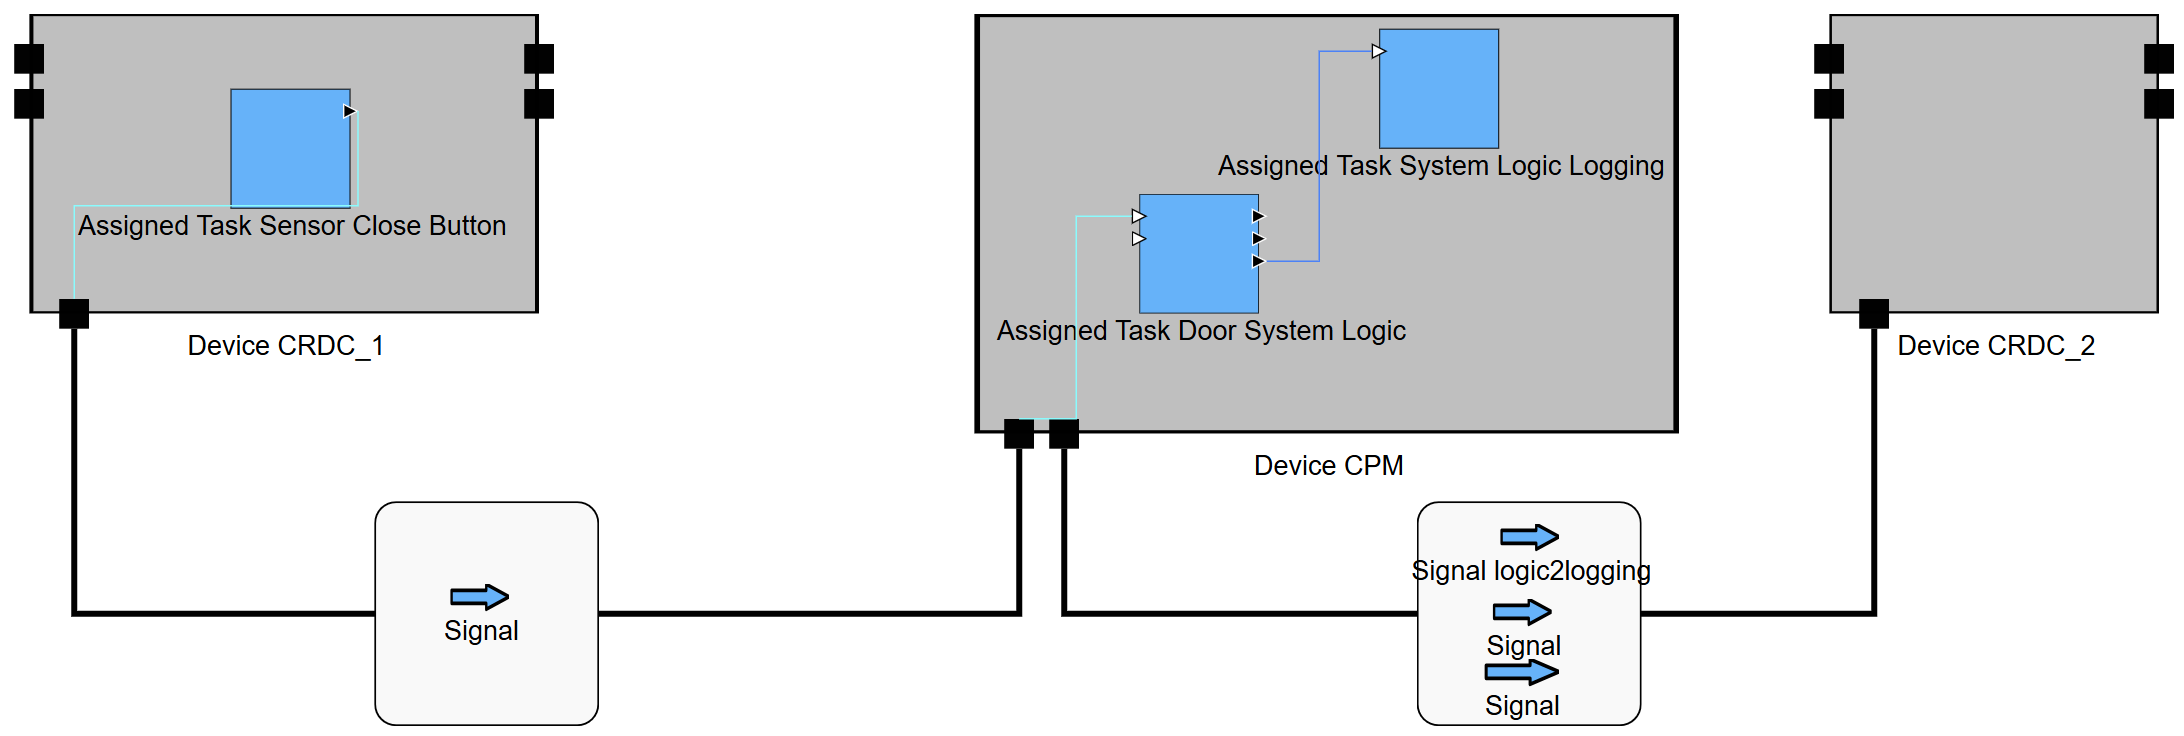
\includegraphics[width=\linewidth]{Pictures/allocations_editor.png}
        \caption{Allocations editor}
        \label{fig_allocations_editor_en}
    \end{subfigure}

    \caption{Functions- Hardware- and Allocations editors}
    \label{fig_editors_en}
\end{figure}
This paper builds upon the work of \cite{og_paper} to automate the verification process within XGEE by tokenizing a screenshot from within the editor. To recognize and process the screenshot data, methods from the "Open Computer Vision" (OpenCV) library are being used.\\
By rebuilding a model from the recognized tokens and comparing it to the original, visualization errors become apparent and can be indicated to the user.
Common visualization errors include:
\begin{itemize}
    \item unclear signal intersections
    \item signals being obscured by blocks
    \item text labels being obscured by signals or blocks
    \item blocks being scaled down to the point of disappearing
    \item blocks obscuring other blocks
\end{itemize}

\section{State of the Art}
\label{sec_state_of_the_art}

The visualization verification tool in \cite{og_paper} could preprocess an automatic screenshot, tokenize edges, vertices and labels, rebuild a model based on the recognized tokens and compare the recognized model with the original.\\
To preprocess the screenshot, the XGEE window is found by searching for the distinct colors of the XGEE title- and status bar and defining the bounding box of the actual block diagram. The grey pixels of the grid are replaced with white, since they are not relevant for the model tokenization.

The vertex detection algorithm was able to detect blue function containers, inputs and outputs with great accuracy, as long as they did not exceed the size limit set by the used template.
The original edge detection algorithm was able to detect edges that went from left to right and from top to bottom with high accuracy. 
The original text detection was using PyTesseract and worked very well, if the text was oriented properly.

\section{Computer Vision}
    
\section{Domain Specific Modeling}

\section{XGEE}

\section{Python}

\section{OpenCV}
\chapter{New Concepts}
\label{chp_new_concepts}
The XGEE visualization verification algorithms are essential for interpreting and optimizing diagram structures within the editor.
While the original implementations demonstrated functionality in basic test cases, their limitations prevented comprehensive detection across various diagram types and complexities. This chapter introduces enhanced methods to address these limitations and significantly increase detection accuracy, versatility and stability.
\section{Edge Detection}
\label{chp_edge_detection}
Edges represent connections between vertices, inputs and outputs. Detecting edges accurately requires an approach that can identify individual line segments and how they connect to form complex chains. This section introduces a robust edge detection pipeline leveraging multiple computer vision techniques to reliably identify edges across a wide variety of block diagrams within XGEE.

\subsection{Methology}
\begin{wrapfigure}{R}{0.4\textwidth}
    \centering
    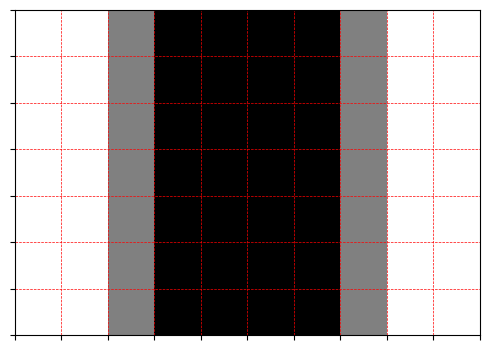
\includegraphics[width=\linewidth]{Pictures/kernel_ver.png}
    \caption{kernel for vertical edges}
    \label{fig_kernel_ver}
\end{wrapfigure}
Since there are only vertical and horizontal edges within XGEE, two kernels will be used to find all pixels containing either part of a vertical or horizontal edge. The \textit{filter2D()} function places the kernel anchor (usually the top left value of the kernel) on top of a pixel, with the rest of the kernel overlapping the corresponding local pixels. The kernel values are then multiplied by the corresponding pixel values underneath and added together. The result is saved and placed on the location of the anchor. The kernel in figure \ref{fig_kernel_ver} is rotated by 90$^{\circ}$ to generate the horizontal kernel. The same process can be expressed using equation \ref{eq_filter2D}, where $H$ is the resulting matrix, $I$ is the original image and $K$ is the used kernel. This process is repeated for every pixel and, depending on the structure of the kernel, it can also be used to blur or sharpen an image \cite{web_filter2D}.\\
Each value in the processed image is normalized to an 8-bit integer between 0 and 255. This allows the data to be visualized as a gray scale image as seen in figure \ref{fig_filter2d} and processed further using OpenCV's \textit{thresholding()} function as in \ref{fig_threshold} to extract the detected pixels.\\
As illustrated in figure \ref{fig_comparison_filter}, ports and letters are sometimes misidentified as edges. Additionally, intersections of edges and points where horizontal and vertical edges meet are not immediately detected. These challenging areas will be processed individually in a later step in the edge detection pipeline. Apart from these specific cases, the method effectively extracts all pixels corresponding to vertical and horizontal edges, provided their widths match those of the used kernels.
\begin{equation}
\label{eq_filter2D}
    H(x, y) = \sum_{i=0}^{M_i-1} \sum_{j=0}^{M_j-1} I(x + i - a_i,y + j - a_j)K(i, j)
\end{equation}

\newpage

\begin{figure}[htb]
    \centering
    \includegraphics[width=1\linewidth]{Pictures/filter2D.png}
    \caption{Filter2D function results}
    \label{fig_filter2d}

    \centering
    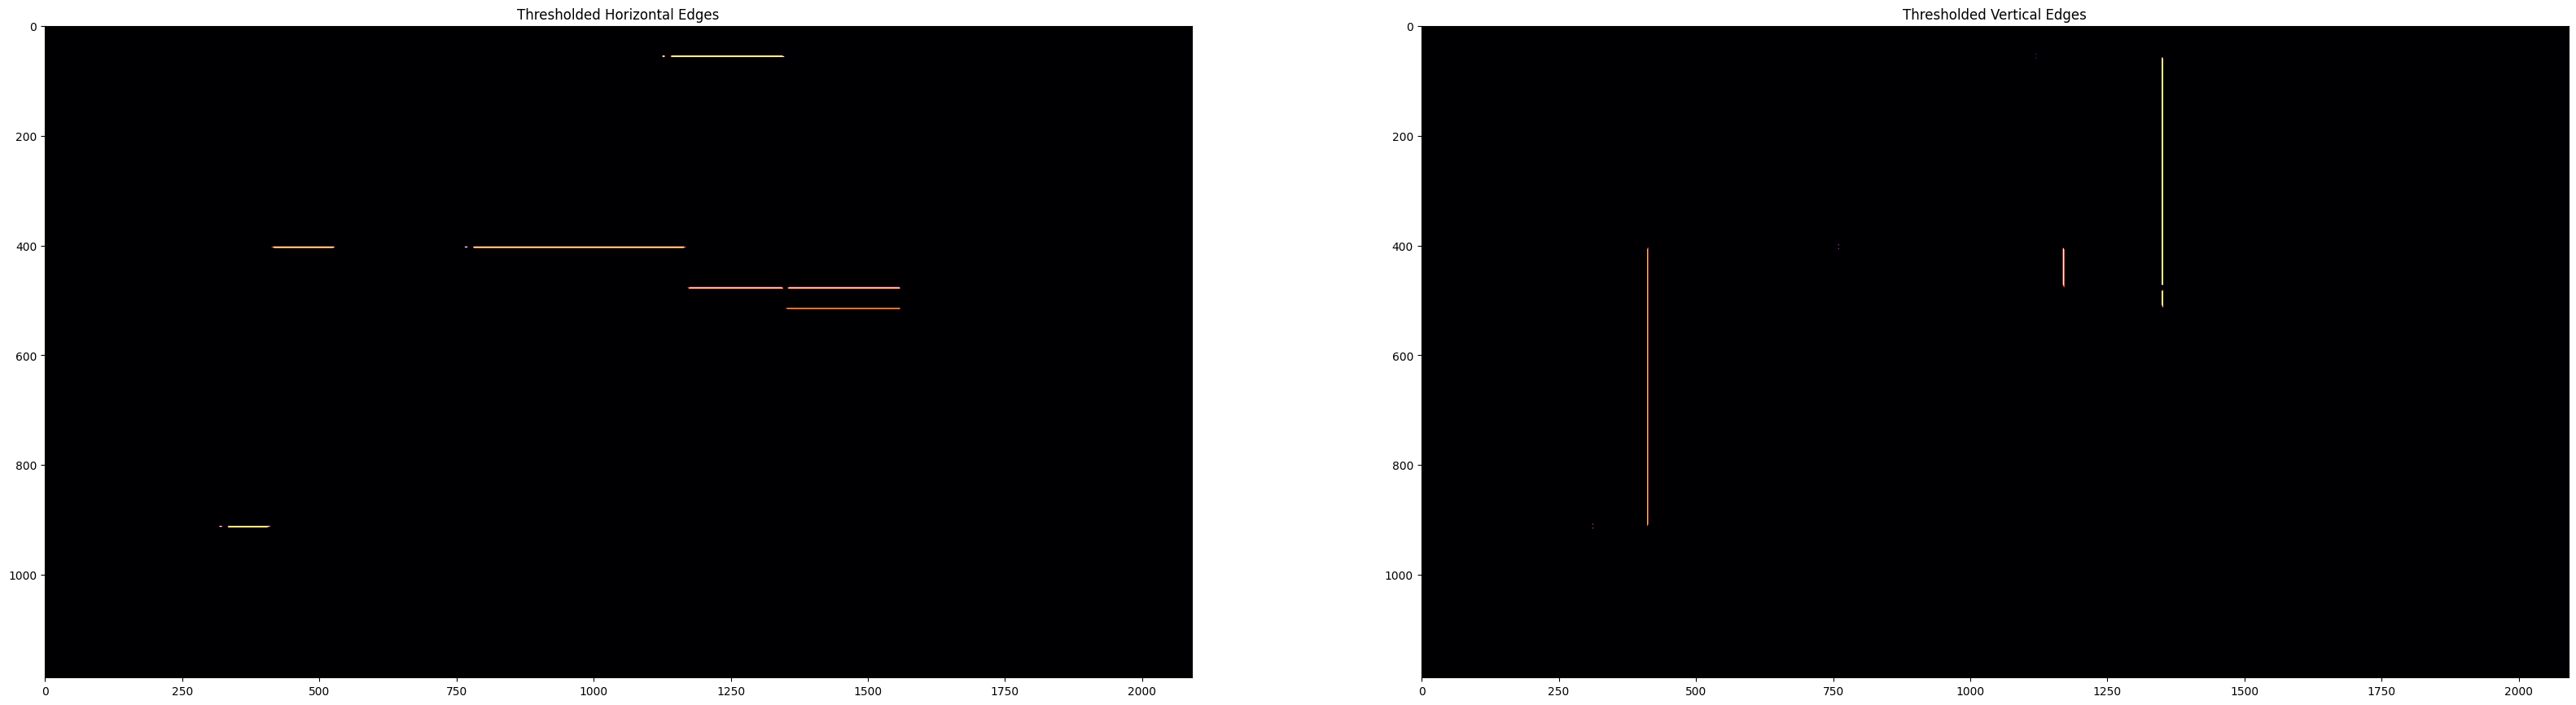
\includegraphics[width=1\linewidth]{Pictures/threshold.png}
    \caption{Thresholded filter2D function results}
    \label{fig_threshold}
\end{figure}
For easier processing and data storage, the thresholded pixels seen in figure \ref{fig_threshold} are converted to line segments consisting of start- and endpoints. This is achieved through two of OpenCV's built-in functions:\\
\textit{findContours()}, which retrieves contours from a binary image using an algorithm introduced by Satoshi Suzuki and others in \cite{art_findContours_algorithm}. In this context, it is used to group nearby pixels and represent them as narrow polygons.\\
\textit{approxPolyDP()}, which approximates a curve or a polygon with another curve or polygon with less vertices using an algorithm introduced by David H Douglas and Thomas K Peucker in their paper: \cite{art_approx_Poly_DP_algorithm}. This function is used to simplify the contours found by \textit{findContours()} into line segments.
\begin{figure}[h]
  \centering
  \begin{minipage}[b]{0.45\textwidth}
    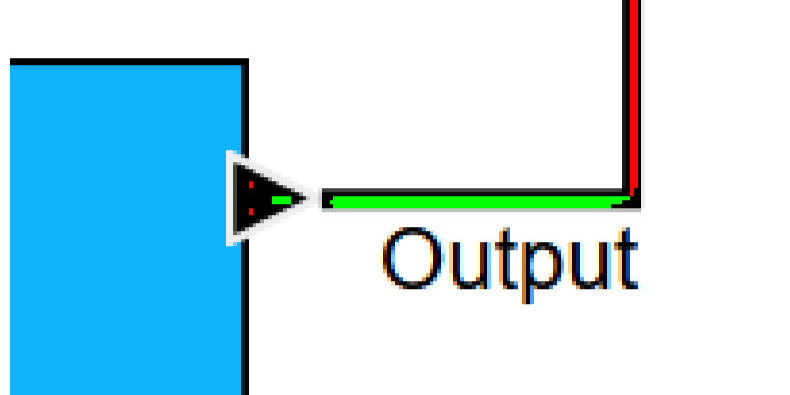
\includegraphics[width=\textwidth]{Pictures/thresh_zoom.png}
  \end{minipage}
  \hfill
  \begin{minipage}[b]{0.45\textwidth}
    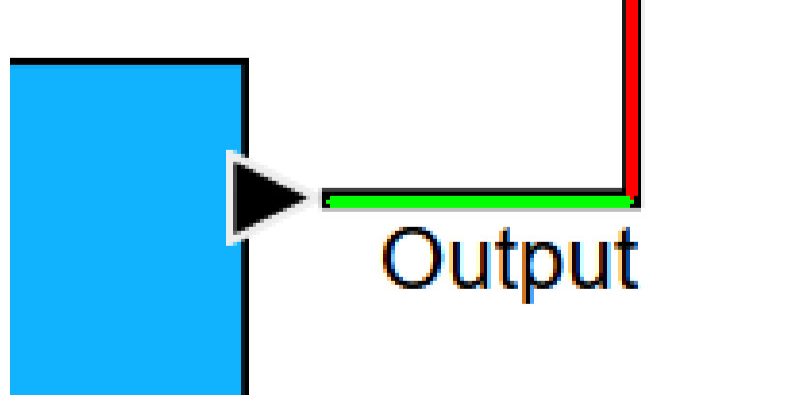
\includegraphics[width=\textwidth]{Pictures/line_segments_zoom.png}
  \end{minipage}
  \caption{Comparison of detected pixels and line segments around an output before and after filtering short segments.}
  \label{fig_comparison_filter}
\end{figure}
\begin{figure}
    \centering
    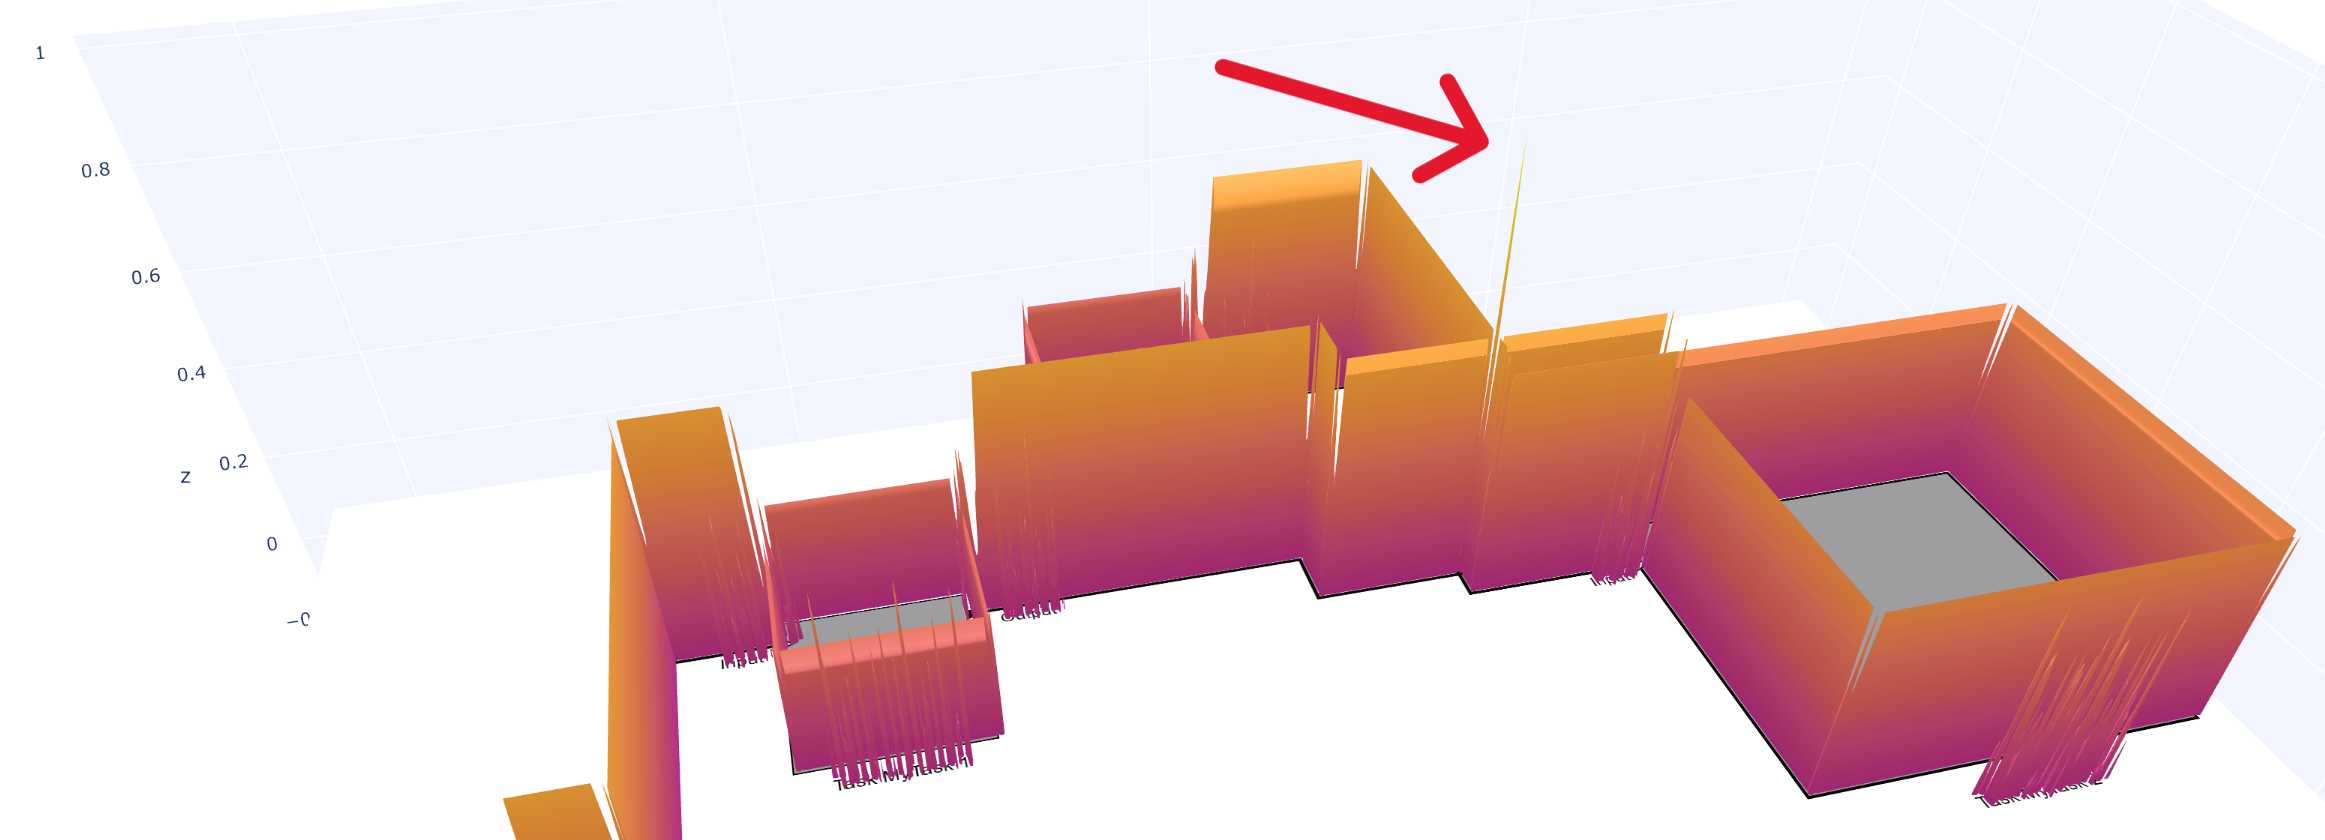
\includegraphics[width=1\linewidth]{Pictures/intersection_peak.png}
    \caption{Simmilarity score peaks at an intersection visualized in 3d using \textit{plotly}.}
    \label{fig_intersection_peak}
\end{figure}\\
Misidentified letters and ports are removed by filtering out all line segments with a length shorter than 20 pixels. In all test cases, this approach successfully removes the unwanted line segments while keeping the edges, illustrated in figure \ref{fig_comparison_filter}.\\
As shown in figure \ref{fig_threshold}, the \textit{filter2D()} function initially does not detect any edges at intersections, leading to gaps between the line segments. To process these gaps, it is assumed that intersections always consist of two straight edges. Overlapping 90$^{\circ}$ turns are considered impossible and will result in an error caused by the incorrect edge recognition. This forces the user to maintain a clear diagram structure.\\
First, all intersections in the image are detected using OpenCV's \textit{matchTemplate()} function, which matches a template image to overlapping regions of the target image \cite{web_matchTemplate}.\\
The function slides the template across the image, comparing overlapping patches with the template using a specified method. Among the available methods \cite{comparison_methods}, tm\_sqdiff\_normed produced the most accurate results. For each pixel, the function calculates and assigns a value representing the similarity between the template and the corresponding image region below. While this approach is more precise than \textit{filter2D()}, it is also significantly more resource-intensive.
% \begin{equation}
% \label{tm_sqdiff_normed}
%     R(x,y) = \frac{\sum_{x', y'}{(T(x', y') - I(x + x', y + y'))^2}}{\sqrt{\sum_{x', y'}{(T(x', y')^2 * \sum_{x', y'}{I(x + x', y + y')^2}}}}
% \end{equation}
At intersections, the similarity value is approximately 85\%. This slight discrepancy likely arises from how modern operating systems use aliasing to render text and lines with higher apparent resolution and contrast compared to the display. Zooming in reveals that the white pixels near edges are often replaced with subtle color hues or shades of gray. Rendering the results of the template matching highlights a peak in similarity at the intersection (Figure \ref{fig_intersection_peak}). Thresholding isolates this peak, typically yielding two or more matches per intersection. These matches are then filtered based on proximity, ensuring only one match is detected at each intersection.\\
The method then processes each detected intersection by connecting the two vertical and two horizontal line segments. This eliminates any residual points near the intersection, leaving only one vertical and one horizontal line segment, illustrated in figure \ref{fig:_intersection_before_after}.\\
In the allocations editor, the same approach is applied to detect and process signal containers on edges. To enhance diagram readability, it is assumed that no 90$^{\circ}$ turns are concealed behind the containers and that edges pass through them in a straight line, avoiding ambiguities that could confuse both computer vision algorithms and human users. The primary distinction from intersection detection lies in the number of line segments: at a signal container, only two line segments meet, rather than four.
\begin{figure}[h]
    \centering
    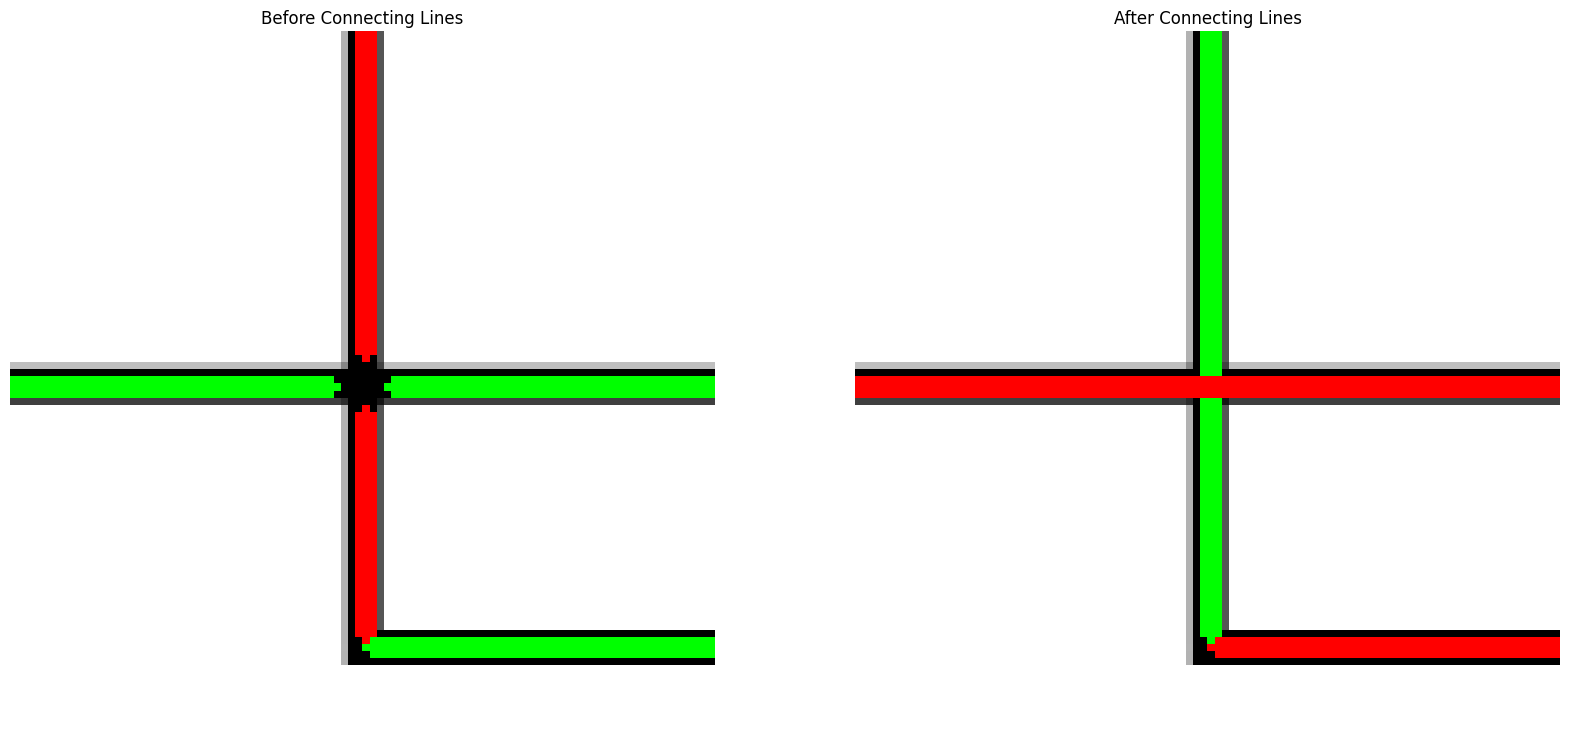
\includegraphics[width=0.7\linewidth]{Pictures/intersection_before_after.png}
    \caption{Intersection before and after connecting the line segments.}
    \label{fig:_intersection_before_after}
\end{figure}\\
Converting the line segments into polylines at this stage would produce unusable data, as the segments are not grouped and not sorted in the sequential order of the edge's \textit{flow}. To generate proper polylines, the line segments must first be sorted into the correct order. For instance, if the first line segment in the list is an intermediate segment within an edge, the polyline function may mistakenly attempt to connect its endpoints directly to the next point in the list, without considering whether it belongs to the same continuous chain, resulting in incorrect edge detections.\\
The implemented method begins by selecting the first line segment, adding it as a starting point to the first chain and to a list of used segments and setting the \textit{chain\_growing} flag to true. It then iterates through the remaining segments, checking whether each segment has already been used and whether any of its points lie within 7 pixels of the endpoints of the current segment. If a match is found, the segment is added to the \textit{used\_segments} list and the current chain. If no segment is found within the 7-pixel threshold, the \textit{chain\_growing} flag is set to false, and the completed chain is added to the list of chains. A threshold of 7 pixels was selected as it reliably produces connected polylines while ensuring that closely positioned lines, such as those at ports, remain distinct and seperate. This process continues until all line segments have been assigned to a chain as in figure \ref{fig_chains_before_after}.
\begin{figure}[h]
    \centering
    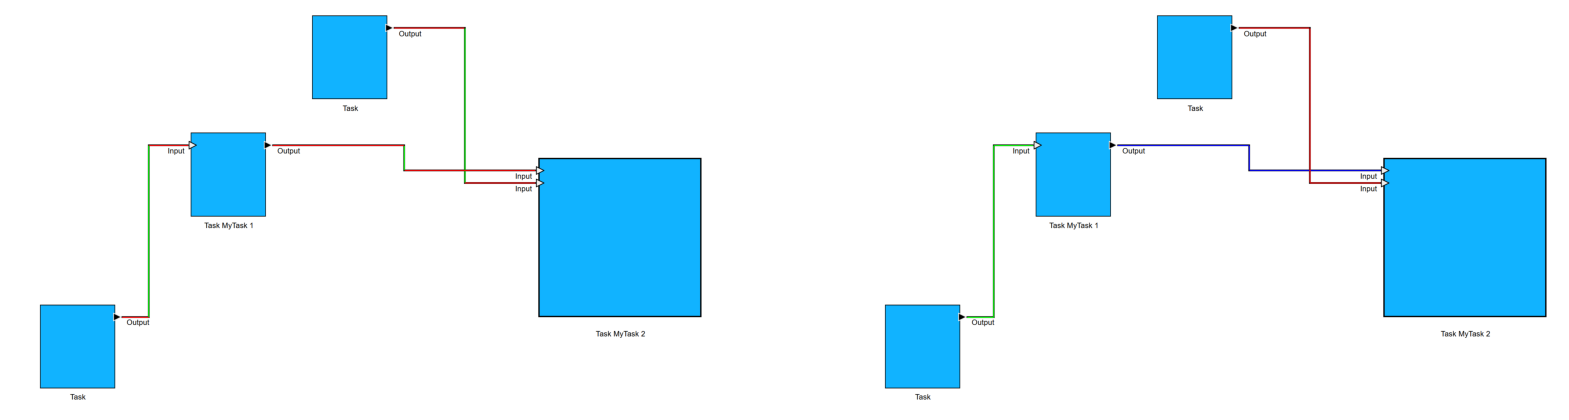
\includegraphics[width=\linewidth]{Pictures/chains_before_after.png}
    \caption{Left: detected vertical and horizontal line segments\\Right: detected line segments grouped into colored line segment chains}
    \label{fig_chains_before_after}
\end{figure}\\
Generating the polylines now would yield better results, but still create unusable data, because the line segments within each chain and the two points within each line segment are not sorted. The first point in a list of line segments in a chain could for example be a point in the middle of the chain, resulting in OpenCV's Polyline function to connect the following points in the wrong order.\\
The sorting algorithm for solving this problem consists of two steps: the first sorts the line segments from the beginning of the chain to the end, the second sorts the end- and startpoint of each line segment individually, so that they too appear in sequential order of 'flow' in the chain.\\
To distinguish between intermediate points and endpoints, the function relies on the method by which the points were initially identified: when two line segments intersect to form a 90$^{\circ}$ degree turn, each segment consists of a start- and an endpoint. As a result, intermediate points in a chain, where line segments meet, always have two points in close proximity, whereas endpoints only have a single point, since only one line segment terminates at each endpoint (see Figure \ref{fig_point_zoom}).
The function leverages this discrepancy by identifying endpoints through an iterative process: It examines each point and checks for the presence of other points within a seven-pixel radius. If no other points are found within this radius, the point is classified as an endpoint of a chain.\\
\begin{figure}
    \centering
    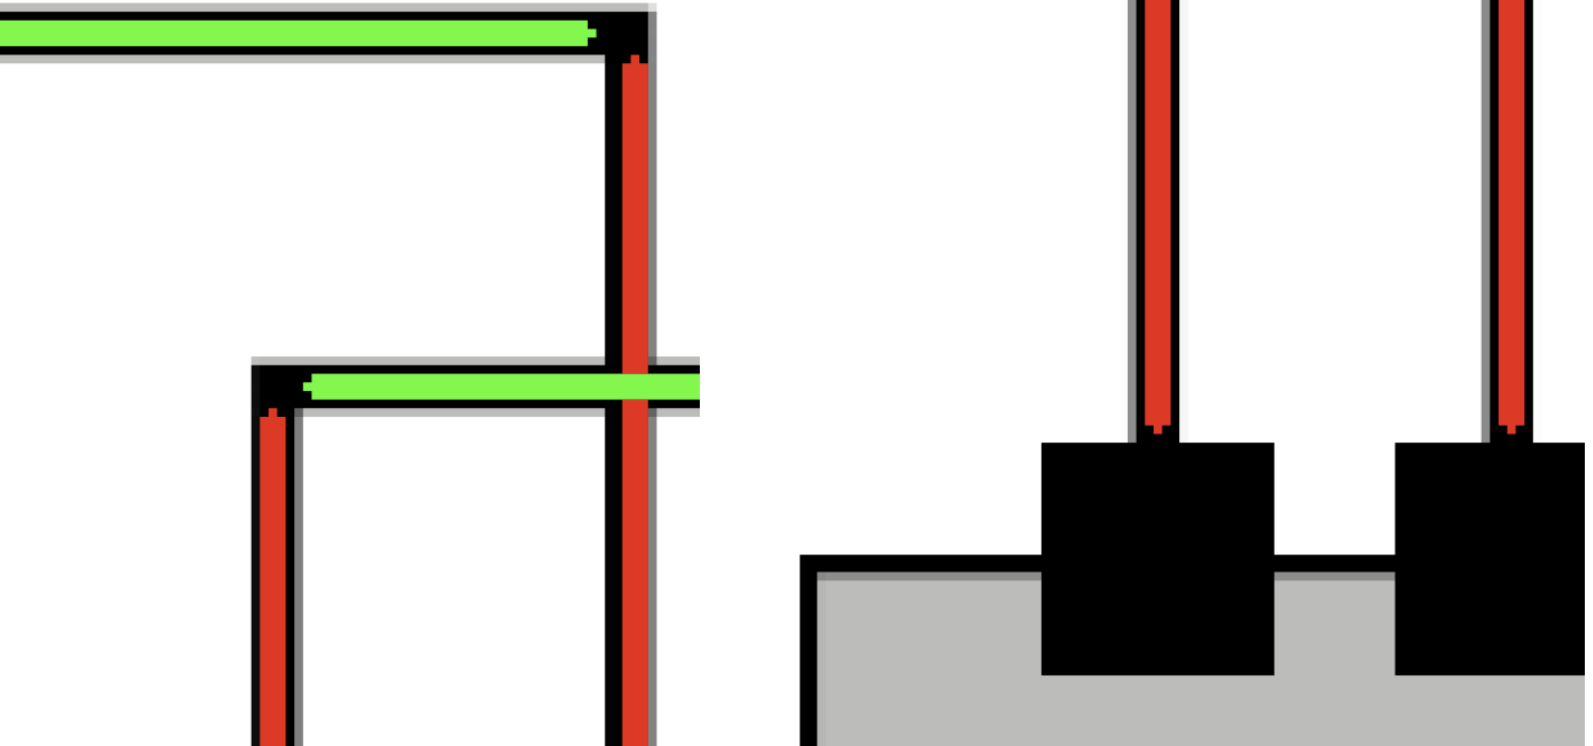
\includegraphics[width=0.5\linewidth]{Pictures/zoomed_in_points.png}
    \caption{Difference between intermediate points and endpoints}
    \label{fig_point_zoom}
\end{figure}
Using the identified endpoints to initialize the \textit{sorted\_chain} list allows the program to organize the chains systematically. The process begins by selecting the segment that includes one of the start points as the initial segment of the chain. The endpoint of this segment that is not a chain endpoint is designated as the first \textit{last\_point} in the \textit{sorted\_chain} list. To determine the next segment in the chain, a \textit{lambda function} calculates the distance between the last point and both points of each remaining segment. The segment containing the point with the smallest distance to the \textit{last\_point} is selected as \textit{next\_segment} and removed from the list of \textit{remaining\_segments}. Within this segment, the point closest to the \textit{last\_point} is appended first to the \textit{sorted\_chain}, followed by the other point of the segment. This process repeats until no segments remain in the \textit{remaining\_segments} list. The entire process is repeated for each chain until all points in all chains are ordered according to the edge's \textit{flow}.

Polylines, which represent connected line segments as ordered lists of points, are a fundamental component in reconstructing edges within the diagram. To generate these polylines from the sorted chains, the method iterates through the \textit{sorted\_chains} list, sequentially appending each point to construct the polylines.The preprocessing of the data ensures that the chains are already structured correctly, making the generation of polylines straightforward and efficient. Once the polyline is constructed, it is converted into the format required by OpenCV for further processing.

\subsection{Further Improvements}
This method successfully detects and processes nearly all edges within XGEE. In contrast to the previous algorithm, it can identify edges in any orientation, regardless of their start or endpoint or order of their line segments. Furthermore, it is capable of processing and interpreting intersections and signal containers, making it well-suited for handling large, complex models. The method performs reliably across all three editor modes, provided the models are formatted correctly.
A notable problem arises when vertices with surrounding black edges are scaled sufficiently, making their edges resemble signal-carrying edges, which complicates their differentiation. In this case, a possible solution would be to let the vertex detection run first and exclude the found areas when applying the edge detection. Alternatively, the presence of colored pixels around the edges could be checked, as the background around edges is typically white, unlike the areas inside device or function vertices. This way, any obstructions caused by the vertices can be avoided.\\
Another issue may arise if the edges are configured by the user in an unexpected way. For instance, intersection within a few pixels of each other or intersections hidden behind vertices cannot be properly interpreted by the current method, which could lead to unexpected results. Future improvements of the XGEE editor, such as a more advanced automatic arrangement algorithm, could reduce or eliminate the risk of ambiguous user input. Additionally, enhancing the readability of subtask edges within the allocations editor would be beneficial for improving the verification tool. Currently, these edges often overlap with text and are thin and have poor contrast, making them difficult for the current edge detection pipeline to detect accurately.

\section{Vertex Detection}
\label{chp_vertex_detection}
Vertices represent distinct visual elements within XGEE such as functions, devices, containers or IO ports. Identifying these vertices is critical for interpreting the structural arrangement of diagrams. This section introduces a template-matching approach to address problems including overlapping vertices and varying sizes, ensuring a more reliable vertex detection in all relevant diagram types within XGEE.

A major problem in template matching is the diversity of vertices within XGEE's three editor models. For example, the functions editor contains only functions, while the hardware editor contains devices and IO ports and the allocations editor contains devices, signal containers, signal arrows and subtasks which overlap with devices and contain their own set of subvertices. Additionally, some vertices are scalable, while others are not. Scalable vertices require extra processing to ensure accurate detection. However, applying this processing universally to all vertices would result in unpredictable and incorrect detections.

\subsection{Methology}
To address these challenges, the list of unique vertices within the current editor model is analyzed to identify any vertices with the \textit{isSubVertexBody}-flag set, which indicates they are subvertices such as subtasks, that overlap with other vertices. These subvertices are prioritized and placed at the beginning of the list of vertices. This way, the vertex detection method can progressively simplify the image by erasing detected subvertices after the first iteration of the vertex detection function, allowing the underlying vertices to be detected without obstruction. Other relevant flags are: 
\begin{itemize}
    \item \textit{isScalable} which indicates whether the vertex can be scaled
    \item \textit{sizeX} and \textit{sizeY} which specify the size of the vertex
    \item \textit{filepath} which specifies the path to the template image
    \item \textit{parent\_filepath} which specifies the path to the parent vertex in case it is a subvertex
\end{itemize}
The method iterates through the list of unique vertices in the current editor model, prioritizing subvertices identified in the previous step. These subvertices are removed from the image by setting all pixels within the bounding box of the subvertex to the \textit{fill} color of the parent vertex as shown in figure \ref{fig_draw_boxes}. This process effectively removes the subvertices from the image, enabling the subsequent vertex detection steps to accurately identify the remaining vertices.\\
\begin{figure}[htb]
    \centering
    \begin{minipage}[b]{0.45\textwidth}
        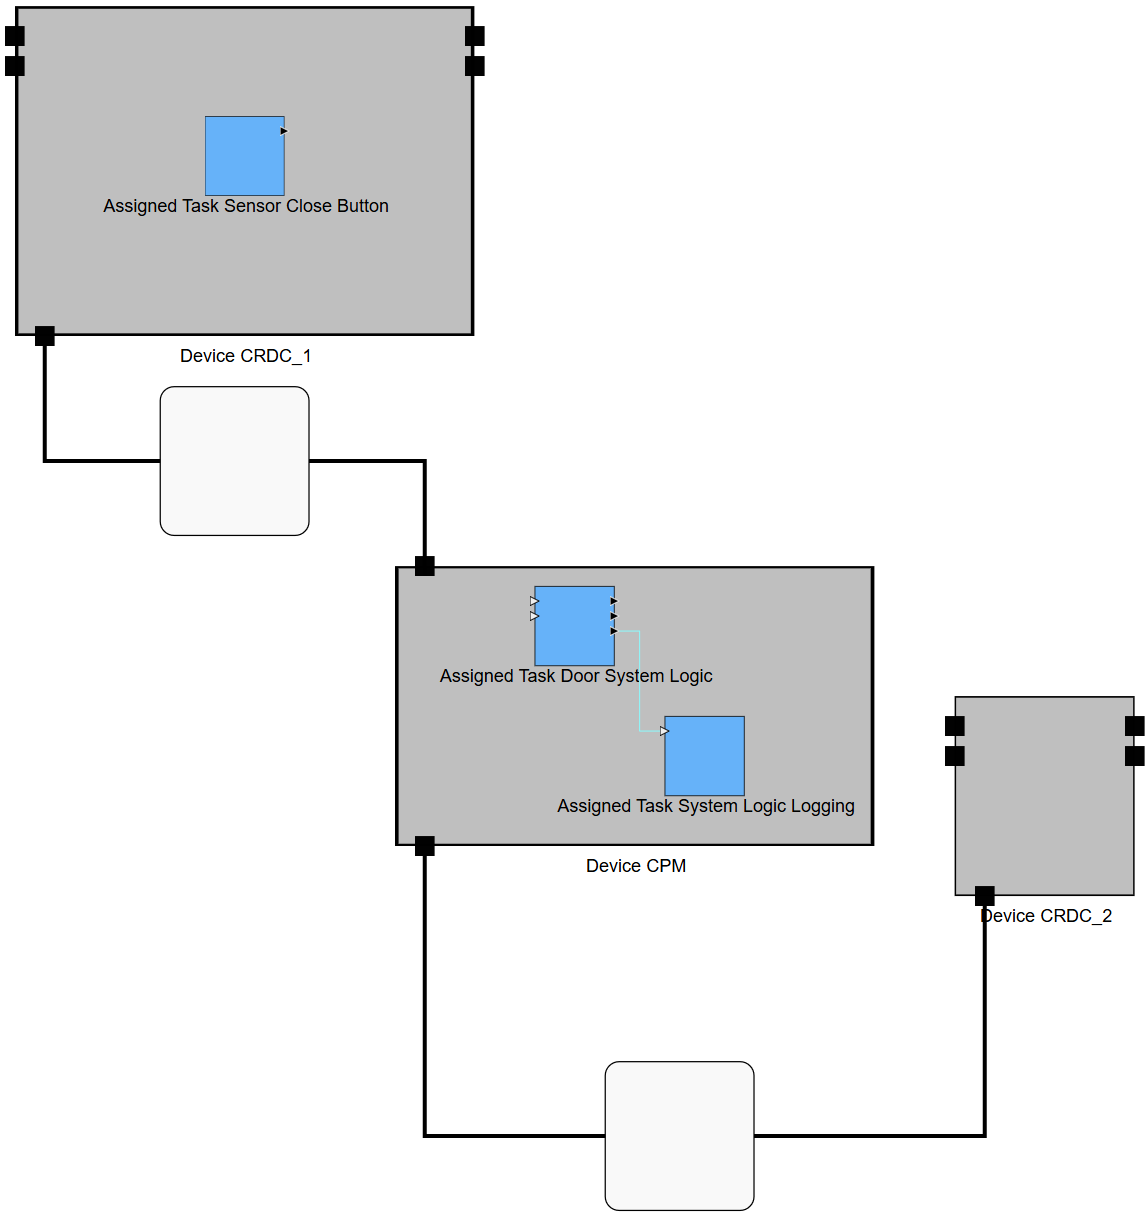
\includegraphics[width=\textwidth]{Pictures/draw_boxes_before.png}
    \end{minipage}
    \hfill
    \begin{minipage}[b]{0.45\textwidth}
        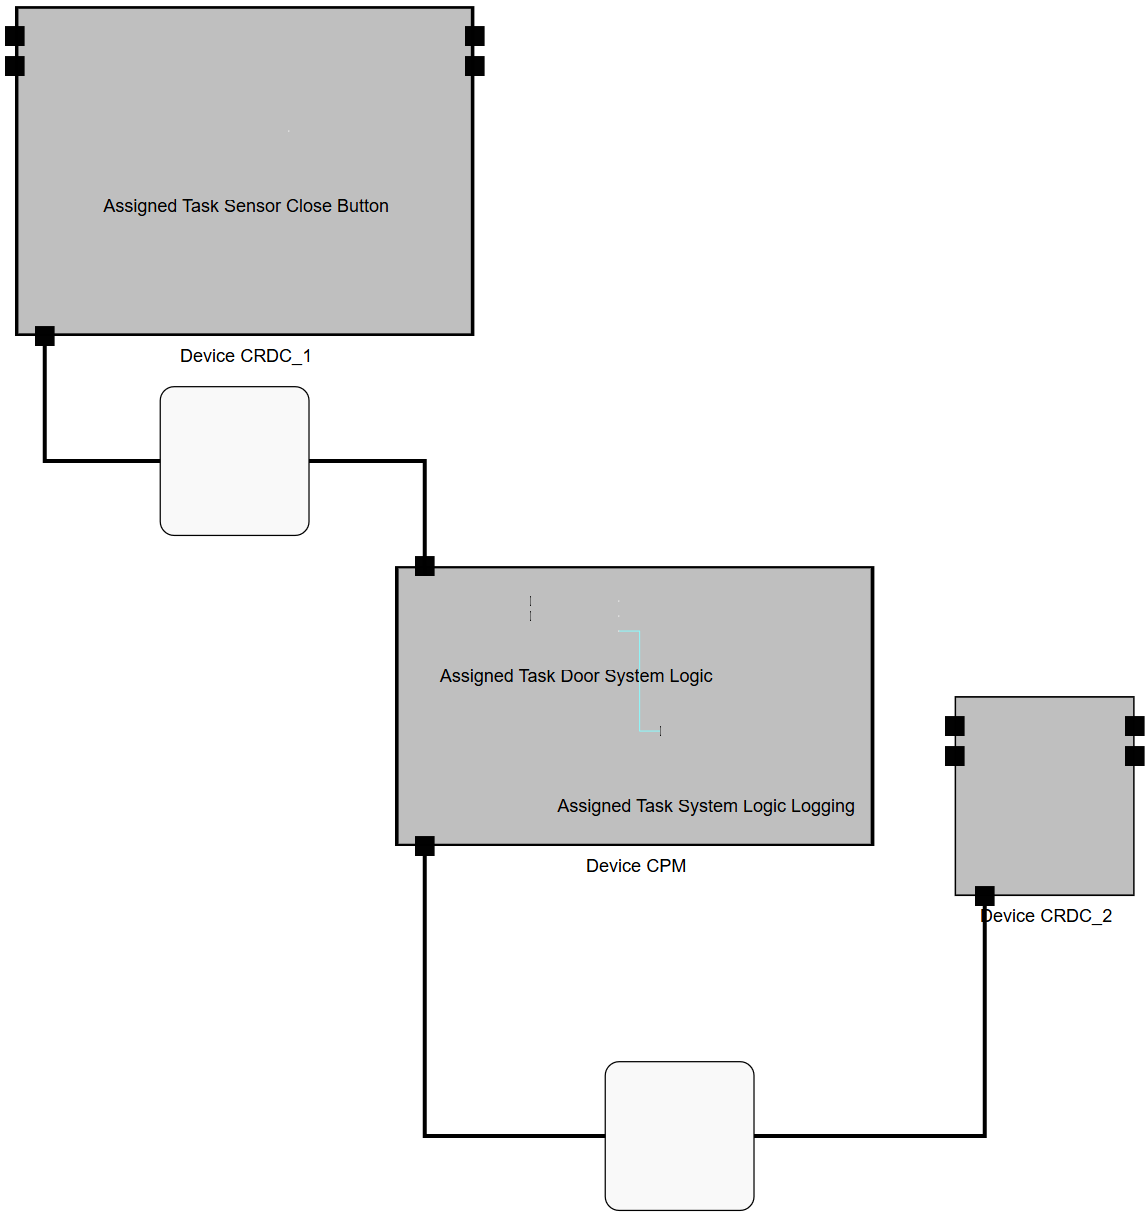
\includegraphics[width=\textwidth]{Pictures/draw_boxes_after.png}
    \end{minipage}
    \caption{Original image from allocations editor containing subvertices (left) and modified image with subvertices removed (right).}
    \label{fig_draw_boxes}
\end{figure}
After processing the subvertices, a new image wrapper object is created using the modified image. The method then iterates through the list of remaining vertices, loading the template image of each vertex using the \textit{filepath} attribute. Depending on the \textit{isScalable} flag, an object of either the \textit{ScalableVertexDetector} or \textit{PortDetector} class is created and the corresponding vertex detection is applied.\\
In case of unscalable vertices, OpenCV's \textit{matchTemplate} and \textit{normalize} functions are applied. The resulting data is thresholded to identify the positions of all found vertices. To define the vertex boundaries, the \textit{sizeX} and \textit{sizeY} attributes are used, allowing bounding boxes of the correct size to be drawn with the detected match serving as the upper-left corner. This approach is effective for detecting vertices like IO ports and subtasks.\\
In case of scalable vertices, this approach does not work because the size of the vertex is not fixed, which reduces the certainty of found matches drastically and eliminates constant \textit{sizeX} and \textit{sizeY} values as a reliable method for defining bounding boxes.\\
Scalable vertices within XGEE are function and device containers that can be resized to improve the readability of visualizations. However, the initial scalable vertex detection algorithm often produced inaccurate results when applied to large function and device containers. Specifically, it tended to produce higher similarity scores at the corners of the container, as the black border surrounding the vertex at these locations more closely resembled the black border in the template image. In contrast, the absence of a black border in the center of the container led to lower similarity scores. In extreme cases, this resulted in the center of the vertex not being detected at all, with the algorithm instead falsely identifying four smaller vertices at the container's corners. The same issue occurred with large devices.\\
To detect these vertices regardless of their dimensions, multiple templates of the same size for different parts of the large vertex as illustrated in figure \ref{fig_templates} are required. They are generated from the (leftmost) original template image by cropping its edges and corners in different ways.
\begin{figure}[h]
    \centering
    
\includegraphics[width=0.85\linewidth]{Pictures/templates.png}
    \caption{Templates for scalable vertex detection generated from the original (leftmost) template image, black edges are exagerated for better visibility.}
    \label{fig_templates}
\end{figure}
Template matching is performed iteratively with each template, comparing the results after each iteration. The highest similarity score for each pixel is retained and combined into the resulting data, which is then thresholded to extract all potential matches.\\
Typically, numerous matches are identified during this process. To eliminate false positives and process the matches to determine the differently sized bounding boxes of the vertices, the algorithm described by Andreas Waldvogel and Björn Annighöfer in \cite{og_paper} is applied.\\
The original image is thresholded to distinguish foreground from background pixels, as illustrated in figure \ref{fig_foreground_threshold}. This foreground information is then utilized to filter the detected matches, retaining only those located within the foreground area. This process effectively removes false positives which often occur because the black pixels along the edges and borders of function or device containers closely resemble those in the black borders in the template images.
\begin{figure}[htb]
    \centering
    \begin{minipage}[b]{0.36\textwidth}
        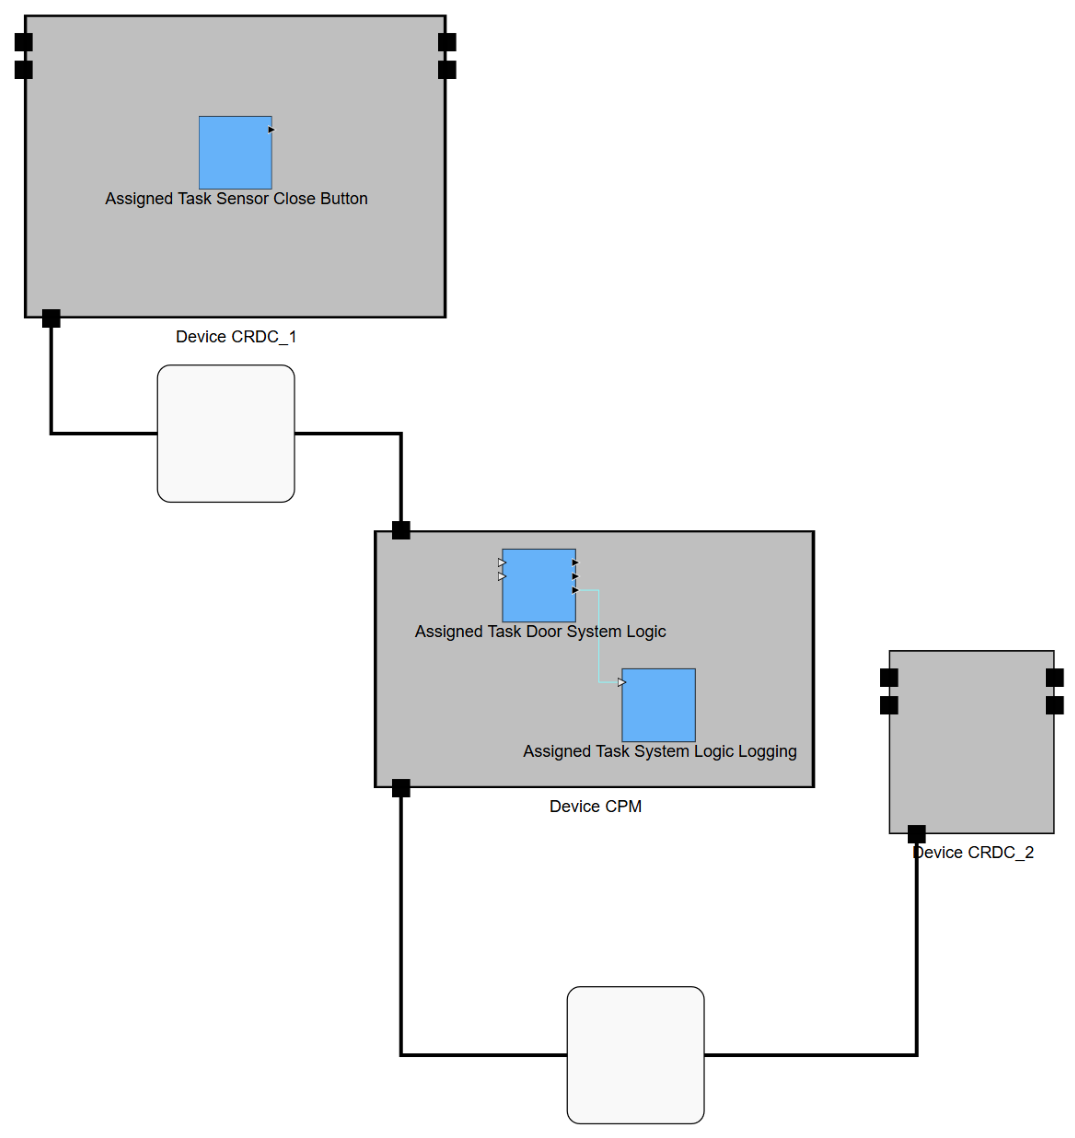
\includegraphics[width=\textwidth]{Pictures/foreground_threshold_before.png}
    \end{minipage}
    \hfill
    \begin{minipage}[b]{0.36\textwidth}
        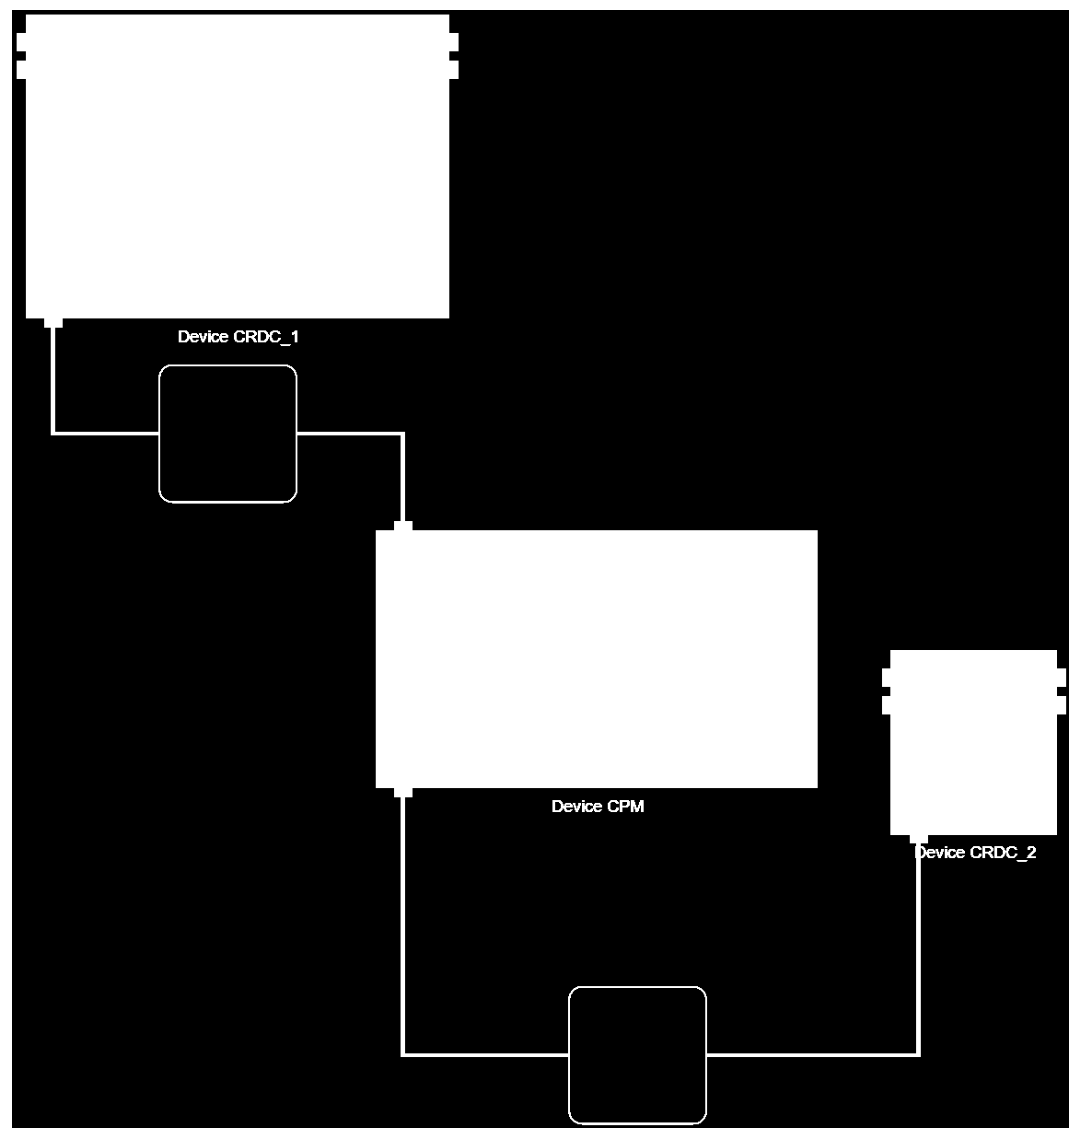
\includegraphics[width=\textwidth]{Pictures/foreground_threshold_after.png}
    \end{minipage}
    \caption{Image from allocations editor (left) with foreground threshold applied (right).}
    \label{fig_foreground_threshold}
\end{figure}\\
For each remaining detected match, the \textit{sizeX} and \textit{sizeY} attributes are used to create a filled bounding box around the detected position. Since multiple matches are often found at various locations within a single large vertex, the overlapping bounding boxes collectively form a larger structure. This structure is then simplified into a single bounding box using OpenCV's \textit{findContours} function.
\begin{figure}[htb]
    \centering
    \begin{minipage}[b]{0.36\textwidth}
        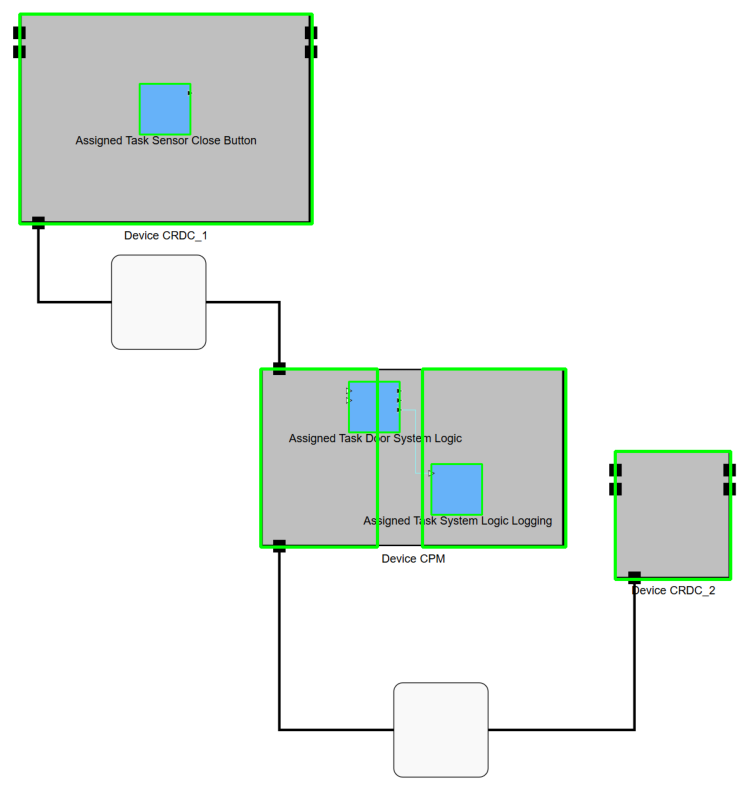
\includegraphics[width=\textwidth]{Pictures/many_templates_before.png}
    \end{minipage}
    \hfill
    \begin{minipage}[b]{0.36\textwidth}
        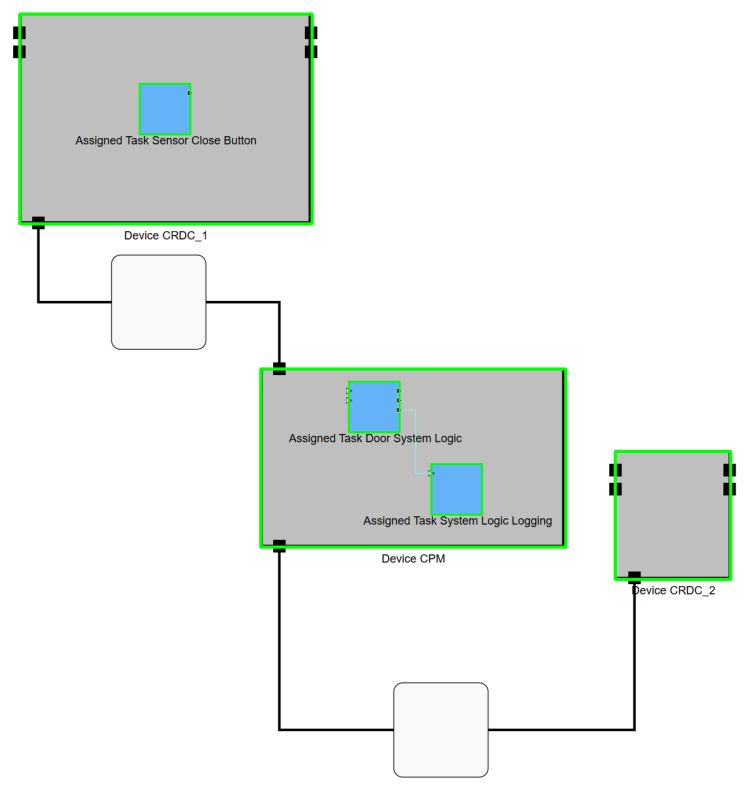
\includegraphics[width=\textwidth]{Pictures/many_templates_after.png}
    \end{minipage}
    \caption{Image from allocations editor containing a large, partially detected device using one template(left) and containing a large, fully detected device using multiple templates(right).}
    \label{fig_many_templates}
\end{figure}
This approach successfully detects all scalable vertices within XGEE, regardless of their dimensions. Using both scalable and non-scalable vertex detection methods ensures that all vertices are detected accurately, regardless of their size or complexity. The method is capable of detecting all vertices in the 10 test cases within this paper, including subvertices and scalable vertices.

\subsection{Further Improvements}
The current method is capable of reliably detecting all vertices within XGEE, including subvertices and scalable vertices. However, enhancing the reliability of subsequent steps in the visualization verification process could be achieved by erasing all detected vertices after processing. To implement this, the method would need to:
\begin{itemize}
    \item Process all vertices in hierarchical top-down order, starting with subvertices and ending with the main vertices.
    \item Dynamically update the input image after each iteration.
    \item Correctly handle cases where subvertices, such as IO ports, only partially overlap with their parent vertices.
\end{itemize}
This approach could also be adapted to erase other components, such as text and edges after their detection, as these elements can interfere with the accurate identification of remaining visualization components.\\
Furthermore, the method could be expanded to detect subvertices of subtasks, which are currently excluded from detection due to their small size. These \textit{subsubvertices} are challenging to differentiate from noise, character fragments, or edge segments using OpenCV. Employing image preprocessing techniques or refining or exchanging the template matching method could improve the detection of these smaller elements.

\section{Text Recognition}
\label{chp_text_recognition}
The original text detection in XGEE utilized Pytesseract, an open-source optical character recognition (OCR) engine developed and sponsored by Google in 2006. Pytesseract required separate installation from other packages and could only detect text in images that had been preprocessed. Additionally, the output data required extensive postprocessing to become usable. While Pytesseract demonstrated high accuracy and speed, it struggled to reliably detect small text or text with low contrast to the background. Its optimization for structured text formats, such as those found in books, further hindered its performance in XGEE, where text can appear in varying orientations, sizes, and positions. These limitations made reliable text detection using Pytesseract difficult to achieve.
\subsection{Methology}
After evaluating various OCR engines, including EasyOCR \cite{easyocr_doc}, Doctr \cite{doctr_doc}, and Keras-OCR \cite{keras_ocr_doc}, EasyOCR proved to be the most suitable alternative.\\
EasyOCR is a deep-learning-based OCR engine that reliably detects text in images, even under challenging conditions such as low contrast or resolution. Although it operates more slowly on modern CPUs compared to some alternatives, it performs significantly faster on GPUs. Additionally, its ability to detect text in multiple languages adds potential value for future applications. Integration of EasyOCR into the XGEE editor for the user is straightforward, as it can be installed directly via pip install easyocr through the requirements.txt file without requiring additional dependencies or downloads. Unlike Pytesseract, EasyOCR only necessitates minimal image preprocessing, and it structures found characters into words and sentences automatically based on proximity, eliminating the need for extensive postprocessing. These advantages make EasyOCR the optimal choice for the updated text detection pipeline within XGEE.

First, a reader object is created and the language of the text is specified. The readtext function of the reader object is then called with the image as an argument. The image has to be padded to have a square shape, so there are no problems rotating the data later. To ensure a more reliable detection, the image is slightly blurred and upscaled to counter any aliasing and small characters. The text detection function then returns a list containing the detected text, its bounding box, and a certainty factor. Parameters can be specified when calling this function to adjust the expected text properties, enhancing the reliability of the detection. For example in earlier versions, EasyOCR struggled to detect single characters, but with these parameter adjustments, this issue has been resolved. The detection process is repeated for the rotated version of the image to ensure comprehensive results. The positions of the bounding boxes of the found rotated text are then rotated around the center of the image to reallign them with the found text of the original image. The found bounding boxes and text are illustrated in figures \ref{fig_text_before} and \ref{fig_text_after}. Reading an image which contains rotated text usually results in many falsely read characters, because for example 'o' and 'l' can be interpreted regardless of orientation. To filter out the falsely read characters, the algorithm first combines the found results of both ocr-searches and then removes every word shorter than three letters.
\begin{figure}[htb]
    \centering
    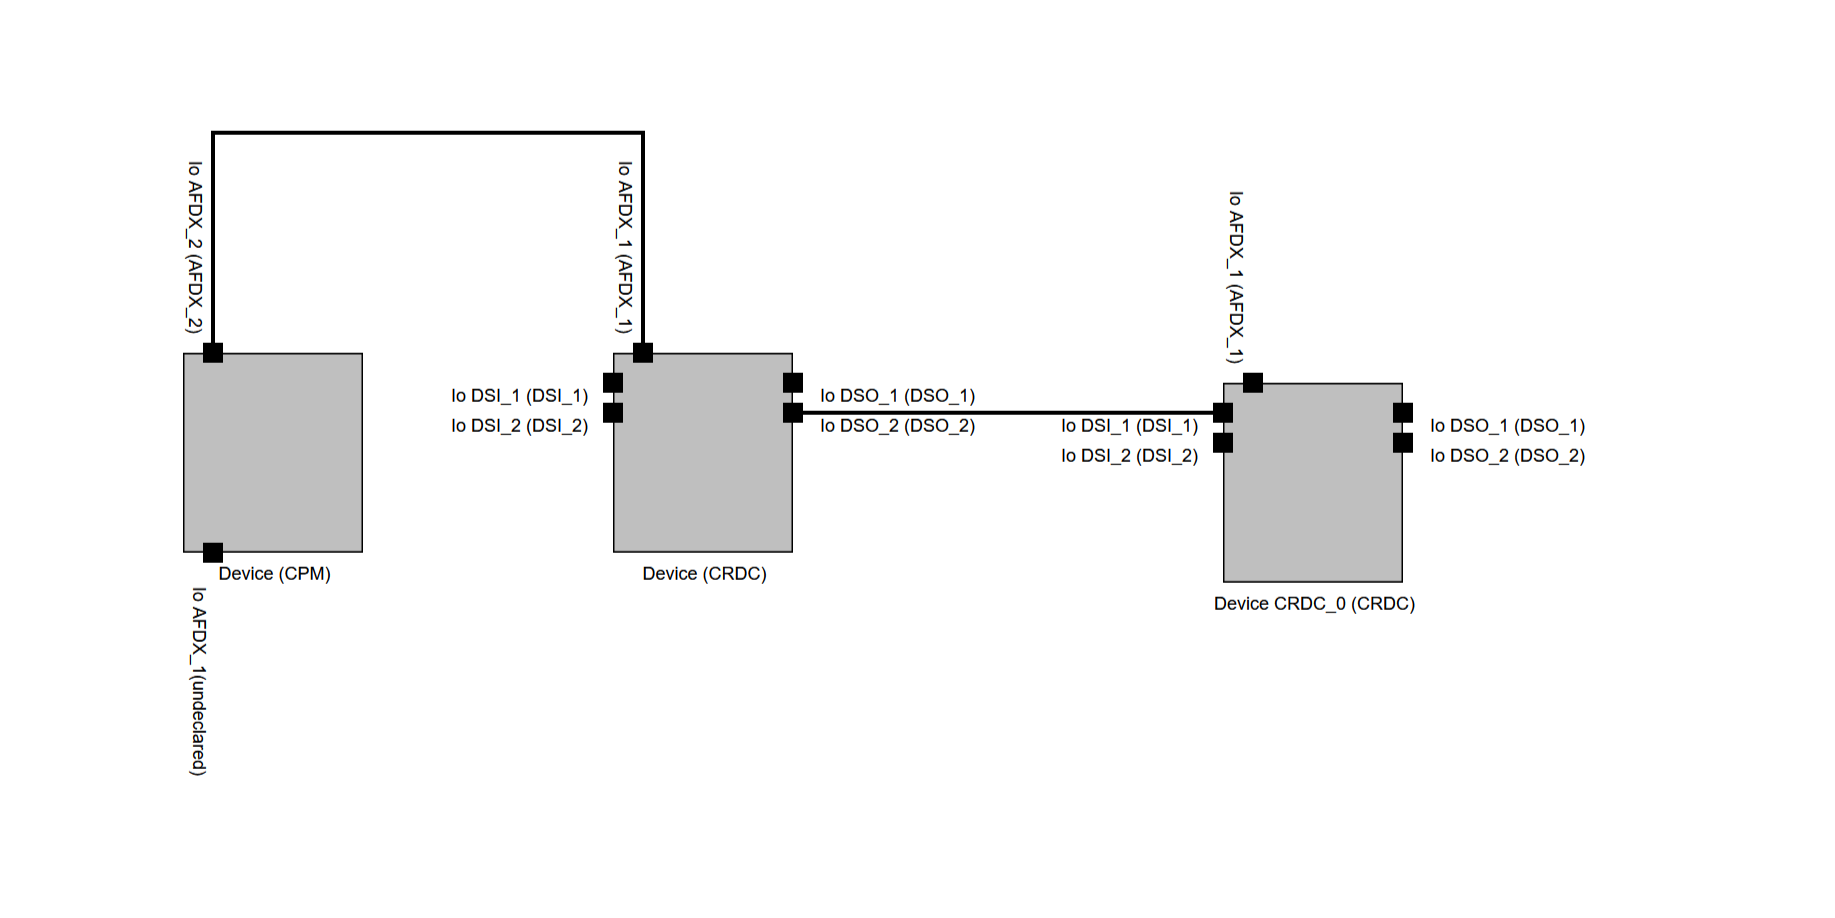
\includegraphics[width=0.8\linewidth]{Pictures/text_before.png}
    \caption{Input image from function editor containing rotated text}
    \label{fig_text_before}

    \centering
    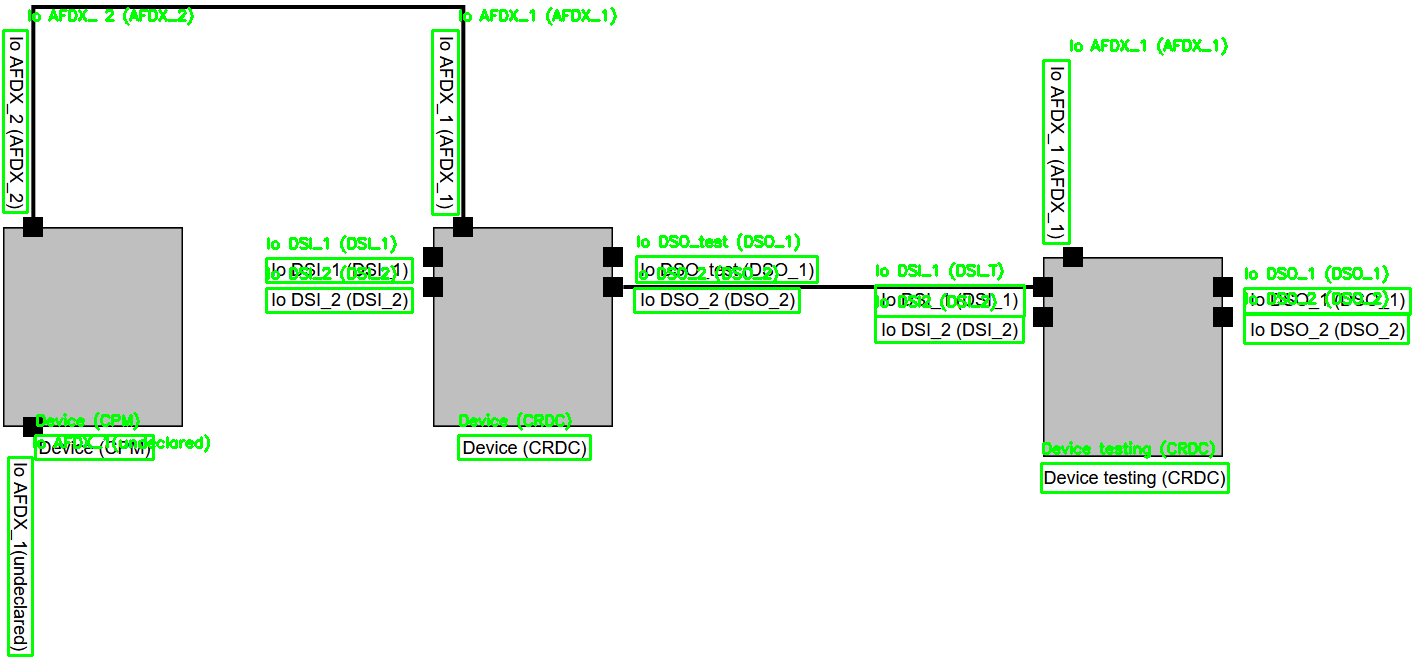
\includegraphics[width=0.8\linewidth]{Pictures/text_after.png}
    \caption{Output image from function editor containing text bounding boxes}
    \label{fig_text_after}
\end{figure}
Because easyocr automatically groups detected characters into words and sentences, this is a simple and effective method to filter out falsely read characters. Using this approach also allows the same algorithm to be used for all models, regardless of the XGEE editor they were created in.
\subsection{Future Improvements}
In the future, this method could be enhanced by incorporating a more advanced algorithm to filter out incorrectly detected characters.\\
Currently, the text recognition is the most time consuming component of the visualization verification process. Optimizing its performance would significantly reduce the overall processing time. This could be achieved by identifying the specific editor type to allow the system to selectively search for rotated characters only when they are expected to be present in the image. Additionally, running the visualization verification on a GPU, parallelizing the text detection to run simultaneous to the edge- and vertex detection or using a more traditional text detection algorithm which does not require as much computational power as EasyOCR would enable the system to process larger models more quickly and efficiently, addressing the current bottleneck in the pipeline.\\

\chapter{Generalization}

\section{Edge Detection}

\section{Vertex Detection}

\section{Text Recognition}

\chapter{Implementation}
\chapter{Demonstration}

\section{Testcases}

\subsection{Testcases 1 - 3}

\subsection{Testcases 4 - 10}

\subsection{Testcases 11 - 15}

\section{Evaluation}
\chapter{Discussion}

\section{Feasability of Proof of Concept}

\section{further improvements}

%% ============================================================
%%  ***  Bibliography
%% ============================================================
\normalem	% Entfernt Unterstrich des Titels
\printbibliography[heading=bibintoc,title=Bibliography] %Literaturverzeichnisse ausgeben

%% ============================================================
%%  ***  Appendix
%% ============================================================
\appendix
% Seitennummerierung wird geändert
\pretocmd{\chapter}{%
	\cleardoublepage
	\pagenumbering{arabic}%
	\renewcommand*{\thepage}{\thechapter\arabic{page}}%
}{}{}
% \chapter{Appendix}
% \label{app:A}

% Beim Aufbau einer Diplomarbeit oder Bachelorarbeit ist der Anhang kein Sammelbecken für alles Übriggebliebene, das im Rahmen der Arbeit gesammelt wurde und für die Bearbeitung der Arbeit nicht relevant war.

% In den Anhang gehören die Materialien, die nicht zwingend für das Textverständnis erforderlich sind. Berechnungen, deren Ergebnisse im Text verwendet wurden, oder der Arbeit zugrundeliegende Fragebögen können hier ausführlicher dargestellt werden \cite{web:studi-lektor}.

% \chapter{Landscape Tabel}\label{app:tabelle-landscape}

% 


% \begin{landscape}


% %	\begin{singlespacing}
% \begin{table}[h]	
% %		\begingroup
% 		\footnotesize
% 		\setlength\tabcolsep{2pt}
% 		\tabulinesep=1mm
% %%		\renewcommand{\arraystretch}{1.4}
% %		
% 	\begin{tabu} to 1.4\textheight{X[l,m,12]X[l,m,4]|X[r,m,10]X[r,m,10]|X[r,m,10]X[r,m,10]|X[r,m,10]X[r,m,10]|X[r,m,10]X[r,m,10]|X[r,m,10]X[r,m,10]|X[r,m,10]X[r,m,10]|X[r,m,10]X[r,m,10]|X[r,m,10]X[r,m,10]|X[r,m,10]X[r,m,10]}
% 		\hline
% 		a & a & a & a & a & a & a & a & a & a & a & a & a & a & a & a & a & a & a & a\\\hline
% %%% Header %%%%% 
% \toprule
% \toprule
% %
% \multicolumn{2}{c|}{Control} & \multicolumn{2}{c|}{load var 1} & \multicolumn{2}{c|}{load var 2} & \multicolumn{2}{c|}{load var 3} & \multicolumn{2}{c|}{load var 4} & \multicolumn{2}{c|}{load var 9} & \multicolumn{2}{c|}{load var 10} & \multicolumn{2}{c|}{load var 13} & \multicolumn{2}{c|}{load var 14} & \multicolumn{2}{c}{overall longitudinal} \\
% \multicolumn{2}{c|}{Surface}  & max. defl. & min. defl. & max. defl. & min. defl. & max. defl. & min. defl. & max. defl. & min. defl. & max. defl. & min. defl. & max. defl. & min. defl. & max. defl. & min. defl. & max. defl. & min. defl. & max. defl. & min. defl. \\
% %
% \midrule
% %
% %\endhead
% %%%%%%%%%%%%%%%%%
% %\bottomrule
% %\bottomrule
% %\endfoot
% %%%%%%%%%%%%%%%%
% %\hline
% %\endlastfoot
% %%%%%%%%%%%%%%%%%%%%%%%%%%%%%%%%%%%%%%%%%%%%%%%%%%%%%%%%%%%%%%%%%%
% %
% %
% \multirow{10}{10mm}{right wing} & 1     & 3.1   & -15.7 & 21.0  & -3.9  & 8.7   & -7.1  & 7.1   & -8.7  & 8.0   & -9.7  & 12.9  & -10.2 & 4.4   & -3.1  & 3.4   & -4.4  & 21.0  & -15.7 \\
%       & 2     & 3.1   & -15.7 & 21.0  & -3.9  & 8.7   & -7.1  & 7.1   & -8.7  & 8.0   & -9.7  & 12.9  & -10.2 & 4.4   & -3.0  & 3.3   & -4.4  & 21.0  & -15.7 \\
%       & 3     & 0.1   & -0.2  & 0.3   & -0.2  & 0.2   & -0.2  & 0.2   & -0.2  & 2.5   & -16.2 & 21.6  & -3.4  & 0.2   & -0.2  & 0.2   & -0.2  & 21.6  & -16.2 \\
%       & 4     & 0.1   & -0.2  & 0.3   & -0.2  & 0.2   & -0.2  & 0.2   & -0.2  & 2.5   & -16.2 & 21.6  & -3.4  & 0.2   & -0.2  & 0.2   & -0.2  & 21.6  & -16.2 \\
%       & 5     & 18.4  & -25.0 & 25.0  & -25.0 & 25.0  & -19.8 & 19.8  & -25.0 & 0.8   & -25.0 & 25.0  & -1.0  & 11.5  & -10.6 & 10.6  & -11.1 & 25.0  & -25.0 \\
%       & 6     & 0.0   & 0.0   & 0.0   & 0.0   & 0.0   & 0.0   & 0.0   & 0.0   & 0.0   & 0.0   & 0.0   & 0.0   & 0.0   & 0.0   & 0.0   & 0.0   & 0.0   & 0.0 \\
%       & 7     & 0.0   & 0.0   & 0.0   & 0.0   & 0.0   & 0.0   & 0.0   & 0.0   & 0.0   & 0.0   & 0.0   & 0.0   & 0.0   & 0.0   & 0.0   & 0.0   & 0.0   & 0.0 \\
%       & 8     & 1.7   & -0.9  & 1.2   & -2.3  & 1.8   & -2.6  & 2.6   & -1.8  & 1.4   & -1.7  & 2.2   & -1.9  & 2.1   & -2.0  & 1.9   & -2.1  & 2.6   & -2.6 \\
%       & 9     & 0.0   & 0.0   & 0.0   & 0.0   & 0.0   & 0.0   & 0.0   & 0.0   & 0.0   & 0.0   & 0.0   & 0.0   & 4.3   & 0.0   & 3.5   & 0.0   & 4.3   & 0.0 \\
%       & 10    & 0.0   & 0.0   & 0.0   & 0.0   & 0.0   & 0.0   & 0.0   & 0.0   & 0.0   & 0.0   & 0.0   & 0.0   & 0.0   & 0.0   & 0.0   & 0.0   & 0.0   & 0.0 \\
% \midrule
% \multirow{10}{10mm}{left wing} & 1     & 3.1   & -15.7 & 21.0  & -3.9  & 8.7   & -7.1  & 7.1   & -8.7  & 8.0   & -9.7  & 12.9  & -10.2 & 4.4   & -3.1  & 3.4   & -4.4  & 21.0  & -15.7 \\
%       & 2     & 3.1   & -15.7 & 21.0  & -3.9  & 8.7   & -7.1  & 7.1   & -8.7  & 8.0   & -9.7  & 12.9  & -10.2 & 4.4   & -3.0  & 3.3   & -4.4  & 21.0  & -15.7 \\
%       & 3     & 0.2   & -0.1  & 0.2   & -0.3  & 0.2   & -0.2  & 0.2   & -0.2  & 2.5   & -16.2 & 21.6  & -3.4  & 0.2   & -0.2  & 0.2   & -0.2  & 21.6  & -16.2 \\
%       & 4     & 0.2   & -0.1  & 0.2   & -0.3  & 0.2   & -0.2  & 0.2   & -0.2  & 2.5   & -16.2 & 21.6  & -3.4  & 0.2   & -0.2  & 0.2   & -0.2  & 21.6  & -16.2 \\
%       & 5     & 18.4  & -25.0 & 25.0  & -25.0 & 25.0  & -19.8 & 19.8  & -25.0 & 0.8   & -25.0 & 25.0  & -1.0  & 11.4  & -10.5 & 10.5  & -11.1 & 25.0  & -25.0 \\
%       & 6     & 0.0   & 0.0   & 0.0   & 0.0   & 0.0   & 0.0   & 0.0   & 0.0   & 0.0   & 0.0   & 0.0   & 0.0   & 0.0   & 0.0   & 0.0   & 0.0   & 0.0   & 0.0 \\
%       & 7     & 0.0   & 0.0   & 0.0   & 0.0   & 0.0   & 0.0   & 0.0   & 0.0   & 0.0   & 0.0   & 0.0   & 0.0   & 0.0   & 0.0   & 0.0   & 0.0   & 0.0   & 0.0 \\
%       & 8     & 0.9   & -1.7  & 2.3   & -1.2  & 2.6   & -1.8  & 1.8   & -2.6  & 1.7   & -1.4  & 1.9   & -2.2  & 2.0   & -2.1  & 2.1   & -1.9  & 2.6   & -2.6 \\
%       & 9     & 0.0   & 0.0   & 0.0   & 0.0   & 0.0   & 0.0   & 0.0   & 0.0   & 0.0   & 0.0   & 0.0   & 0.0   & 4.3   & 0.0   & 3.5   & 0.0   & 4.3   & 0.0 \\
%       & 10    & 0.0   & 0.0   & 0.0   & 0.0   & 0.0   & 0.0   & 0.0   & 0.0   & 0.0   & 0.0   & 0.0   & 0.0   & 0.0   & 0.0   & 0.0   & 0.0   & 0.0   & 0.0 \\
% \bottomrule
% \bottomrule

% \multicolumn{20}{l}{Control Functions:} \\
% \multicolumn{20}{l}{Pitch: 1 \& 2; Roll: 3 \& 4; Stabilisation: 5; Spliteron: 6; Miniflap: 7; Rudder: 8; Inner Spoiler: 9; Outer Spoiler: 10} \\
% \multicolumn{20}{l}{Note: The Control Surfaces 6 and 7 are not operational within the MATLAB SIMULINK models.} \\		
% 		\end{tabu}
% \caption{Control surface deflections at longitudinal manoeuvres}\label{tab:Flap-Deflections}
% \end{table}
% %		\endgroup

% %	\end{singlespacing}

% \end{landscape}
% \normalsize




% \chapter{Long Table}\label{app:mehrsteige-tabelle}

% % \begin{longtabu} to \textwidth{|X[l,m,1]|X[l,m,1]|X[l,m,1]|}

	
% 	\toprule\toprule \multicolumn{1}{|c|}{\textbf{First column}} & \multicolumn{1}{c|}{\textbf{Second column}} & \multicolumn{1}{c|}{\textbf{Third column}} \\ \midrule 
% 	\endfirsthead
	
% 	\multicolumn{3}{c}%
% 	{\tablename\ \thetable{} -- continued from previous page} \\
% 	\toprule\toprule \multicolumn{1}{|c|}{\textbf{First column}} & \multicolumn{1}{c|}{\textbf{Second column}} & \multicolumn{1}{c|}{\textbf{Third column}} \\ \midrule 
% 	\endhead
	
% 	\midrule \multicolumn{3}{|r|}{{Continued on next page}} \\ \bottomrule\bottomrule
% 	\caption[]{A sample long table} \label{tab:long} \\
% 	\endfoot
	
% 	\bottomrule
% 	\bottomrule
% 	\caption[A sample long table]{A sample long table} \label{tab:long} \\
% 	\endlastfoot
	
% 	One & abcdef ghjijklmn & 123.456778 \\
% 	One & abcdef ghjijklmn & 123.456778 \\
% 	One & abcdef ghjijklmn & 123.456778 \\
% 	One & abcdef ghjijklmn & 123.456778 \\
% 	One & abcdef ghjijklmn & 123.456778 \\
% 	One & abcdef ghjijklmn & 123.456778 \\
% 	One & abcdef ghjijklmn & 123.456778 \\
% 	One & abcdef ghjijklmn & 123.456778 \\
% 	One & abcdef ghjijklmn & 123.456778 \\
% 	One & abcdef ghjijklmn & 123.456778 \\
% 	One & abcdef ghjijklmn & 123.456778 \\
% 	One & abcdef ghjijklmn & 123.456778 \\
% 	One & abcdef ghjijklmn & 123.456778 \\
% 	One & abcdef ghjijklmn & 123.456778 \\
% 	One & abcdef ghjijklmn & 123.456778 \\
% 	One & abcdef ghjijklmn & 123.456778 \\
% 	One & abcdef ghjijklmn & 123.456778 \\
% 	One & abcdef ghjijklmn & 123.456778 \\
% 	One & abcdef ghjijklmn & 123.456778 \\
% 	One & abcdef ghjijklmn & 123.456778 \\
% 	One & abcdef ghjijklmn & 123.456778 \\
% 	One & abcdef ghjijklmn & 123.456778 \\
% 	One & abcdef ghjijklmn & 123.456778 \\
% 	One & abcdef ghjijklmn & 123.456778 \\
% 	One & abcdef ghjijklmn & 123.456778 \\
% 	One & abcdef ghjijklmn & 123.456778 \\
% 	One & abcdef ghjijklmn & 123.456778 \\
% 	One & abcdef ghjijklmn & 123.456778 \\
% 	One & abcdef ghjijklmn & 123.456778 \\
% 	One & abcdef ghjijklmn & 123.456778 \\
% 	One & abcdef ghjijklmn & 123.456778 \\
% 	One & abcdef ghjijklmn & 123.456778 \\
% 	One & abcdef ghjijklmn & 123.456778 \\
% 	One & abcdef ghjijklmn & 123.456778 \\
% 	One & abcdef ghjijklmn & 123.456778 \\
% 	One & abcdef ghjijklmn & 123.456778 \\
% 	One & abcdef ghjijklmn & 123.456778 \\
% 	One & abcdef ghjijklmn & 123.456778 \\
% 	One & abcdef ghjijklmn & 123.456778 \\
% 	One & abcdef ghjijklmn & 123.456778 \\
% 	One & abcdef ghjijklmn & 123.456778 \\
% 	One & abcdef ghjijklmn & 123.456778 \\
% 	One & abcdef ghjijklmn & 123.456778 \\
% 	One & abcdef ghjijklmn & 123.456778 \\
% 	One & abcdef ghjijklmn & 123.456778 \\
% 	One & abcdef ghjijklmn & 123.456778 \\
% 	One & abcdef ghjijklmn & 123.456778 \\
% 	One & abcdef ghjijklmn & 123.456778 \\
% 	One & abcdef ghjijklmn & 123.456778 \\
% 	One & abcdef ghjijklmn & 123.456778 \\
% 	One & abcdef ghjijklmn & 123.456778 \\
% 	One & abcdef ghjijklmn & 123.456778 \\
% 	One & abcdef ghjijklmn & 123.456778 \\
% 	One & abcdef ghjijklmn & 123.456778 \\
% 	One & abcdef ghjijklmn & 123.456778 \\
% 	One & abcdef ghjijklmn & 123.456778 \\
% 	One & abcdef ghjijklmn & 123.456778 \\
% 	One & abcdef ghjijklmn & 123.456778 \\
% 	One & abcdef ghjijklmn & 123.456778 \\
% 	One & abcdef ghjijklmn & 123.456778 \\
% 	One & abcdef ghjijklmn & 123.456778 \\
% 	One & abcdef ghjijklmn & 123.456778 \\
% 	One & abcdef ghjijklmn & 123.456778 \\
% 	One & abcdef ghjijklmn & 123.456778 \\
% 	One & abcdef ghjijklmn & 123.456778 \\
% 	One & abcdef ghjijklmn & 123.456778 \\
% 	One & abcdef ghjijklmn & 123.456778 \\
% 	One & abcdef ghjijklmn & 123.456778 \\
% 	One & abcdef ghjijklmn & 123.456778 \\
% 	One & abcdef ghjijklmn & 123.456778 \\
% 	One & abcdef ghjijklmn & 123.456778 \\
% 	One & abcdef ghjijklmn & 123.456778 \\
% 	One & abcdef ghjijklmn & 123.456778 \\
% 	One & abcdef ghjijklmn & 123.456778 \\
% 	One & abcdef ghjijklmn & 123.456778 \\
% 	One & abcdef ghjijklmn & 123.456778 \\
% 	One & abcdef ghjijklmn & 123.456778 \\
% 	One & abcdef ghjijklmn & 123.456778 \\
% 	One & abcdef ghjijklmn & 123.456778 \\
% 	One & abcdef ghjijklmn & 123.456778 \\
% \end{longtabu}
\end{document}
